\documentclass[UTF8]{ctexart}

\usepackage{amsmath}
\usepackage{hyperref}
\usepackage{graphicx}
\usepackage{listings}
\usepackage{subfigure}
\usepackage{float}


\title{muon 模拟}

\begin{document}

\section{研究背景介绍}
\subsection{蒙特卡罗模拟}

蒙特卡罗(Monte Carlo 简写 MC)方法,又称计算机随机模拟方法,是一种基于”随机数“的计算方法。该方法最早用于第二次世界大战时美国洛斯阿拉莫斯实验室(LANL)的”曼哈顿计划“中设计核武器的统计计算,由该计划的主持人之一的数学家冯诺依曼(John von Neumann) 用闻名世界的赌城摩纳哥 Monte Carlo 命名。蒙特卡洛进行的实验,具体而言,是基于所针对问题的概率模型、几何数量以及几何特征,沿承着模型中实验的过程,通过数学模拟实验对已有的概率分布进行抽样分析,由此获得模拟量的实验方法。\\

随着计算机的性能的提高和蒙特卡罗方法研究的深入和应用范围的扩大,探测器的模拟成为可能。目前高能物理领域的粒子探测系统结构愈发复杂,而这种复杂性的增加使得在预测某种趋势或者进行某种计算的时候需要使用蒙特卡洛模拟的方法。尽管在粒子探测的模拟中,可以通过对于主要信息的辐射方程以及输运方程进行构建和求解,但是使用蒙特卡洛模拟显然可以简化此类步骤。相比之下,蒙特卡洛方法更关注概率统计模型的构建,而主要操作——使用随机数(或伪随机数)对随机变量抽样,以及多次重复实验的工作,大多都由计算机完成。之后在根据获得的大量的实验结果,根据模型的规则,使用数学方法明确出数据中隐藏的特性。总体上,基于统计学的思想获得所求解的数学期望等值,以此来表示实验可能出现的结果。\\

同时模拟探测器的原因是为了对探测器性能进行优化,确定数据获取中触发判断选择逻辑,估计实验所能达到的物理目标以及解释预测实验结果,因此模拟程序必须精确地描述探测器的几何结构,模拟粒子与探测器介质的物理过程,以获得一定程度可以信服的模拟结果。由于我们的缪子探测器,正在搭建过程中,急需对探测器的结构进行优化,为此我们搭建了基于Geant4开发的探测器模拟程序。

\subsection{Geant4介绍}

Geant4是欧洲核子中心(CERN)新近研制开发的一个大型高能物理探测器模拟程序,是采用当代先进的面向对象程序设计技术利用C++语言编写的。\cite{1}该软件包提供了高能物理模拟实验探测器的必要工具,利用探测器几何结构的相关类,用户能够精确地定义复杂探测器的材料和几何结构,利用物理过程的相关类,通过对不同粒子注册相关的物理过程,用户能够模拟所有己知的粒子与探测器介质之间的各种可能的相互作用,同时可以用不同可视化引擎查看探测器的几何结构以及粒子在探测器中的径迹,方便初学者了解探测器模拟。同时用户可以定义不同的“动作”(Action)类来控制模拟过程相应的层面的行为或者输出所产生的数据。
\subsection{缪子探测的教学意义}

我们在Geant4的基础上设计了缪子探测系统,用以指导探测缪子实际装置的搭建,以测量缪子寿命。在缪子寿命实验中,涉及的理论知识与技术涵盖了高能物理实验的几乎各个环节,例如粒子的来源、探测器设计与模拟,核电子学,探测器与电子学刻度,在线获取系统和数据离线分析等方法与技术。\cite{2}所以对缪子寿命测量具有重要物理意义和教学意义,比如利用缪子寿命精确值来确定粒子物理标准模型中的费米耦合常量;验证狭义相对论中的时间膨胀效应。

\section{缪子探测器基本工作原理}
\subsection{缪子简介}

缪子是一种类似电子的基本粒子,它带有一个单位负电荷,自旋为$\frac{1}{2}$,但是相比电子,质量更大,为$105. 658MeV/c^2$,是电子的207倍重,被分类为轻子。和其他轻子一样,缪子被认为没有子结构。缪子的反粒子为$\mu^+$,带有一个单位正电荷。\cite{3}缪子的平均寿命约为$2.2\mu s$, 准确值为 2.1969811(22)×10−6 s,缪子的衰变方式: \cite{4}\\
\begin{align}
\mu^- \rightarrow e^- + \nu_\mu + \bar\nu_e\\
\mu^+ \rightarrow e^+ + \bar\nu_\mu + \nu_e
\end{align}

到达地球表面的缪子绝大部分不是来自宇宙射线,而是由宇宙射线中高能质子撞击大气层顶部,产生 $\pi$ 介子,然后 $\pi$ 介子会在传输较短的距离后衰变,产生缪子($\pi^- \rightarrow \mu^- + \bar{\nu_u} ,\ \pi^+\rightarrow \mu^+ + \nu_\mu$)。如果不考虑相对论效应,这些缪子的寿命大约能够支持传输468米(2.197 µs×ln(2) × 0.9997×c),但是由于相对论效应的时钟变慢效应,这些缪子就能够达到地球表面。\cite{3}

\subsection{塑料闪烁体}

闪烁体分有机闪烁体(塑料闪烁体,蒽,液体闪烁体)和无机闪烁体(NaI,CsI,溴化镧等),塑料闪烁体是有机闪烁物质在塑料中的固溶体,通常由基质、闪烁物质及移波剂组成,塑料闪烁体中的基质(例聚苯乙烯)起着能量转移作用,能吸收能量,然后转移给闪烁分子,使闪烁效率提高。移波剂是用来改变光的波长,使闪烁体输出的光能更好地在光电倍增管的光阴极上打出光电子,改善闪烁探测器的信号输出。

\subsection{光电倍增管}

光电倍增管是一个电真空器件,它由光阴极、若干个倍增电极和个阳极组成。光阴极前有一个玻璃或者石英制成的窗,整个器件外壳为玻璃,各电极由针脚引出。通过高压电源和分压电阻,使阳极--各个倍增电极--阴极间建立从高到低的电位分布。当闪烁光子入射到光阴极上,由于光电效应会产生光电子,这些光电子受极间电场加速和聚焦,打在第一个倍增电极上,产生个二次电子,这些二次电子在以后各级倍增电极上又发生同样的倍增过程,直到最后在阳极上可接收到$10^4-10^9$个电子。所以人们把这种器件称为光电倍增管。大量电子会在阳极负载上建立起电信号,通常为电流脉冲或电压脉冲,然后通过起阻抗匹配作用的射极跟随器,由电缆将信号传输到电子学仪器中去。\\

光电倍增管具有增益高和响应时间短,输出电流和入射光子数成正比的特性,但是由于极间的欧姆漏阻、阴极或其他部件的热电子发射以及残余气体的离子发射、场致发射和玻璃闪烁,可能存在暗电流,这是光电倍增管的本底噪声。

\subsection{符合法测量宇生缪子}

在粒子物理实验中 ,对于平均寿命大于 $10^{-9}s$的不稳定粒子, 传统的粒子寿命测量方法是直接测量衰变事例的时间分布, 计算出粒子的寿命.实验上通常采用延迟符合法测量$\mu$子的平均寿命.该方法至少需要 2 个探测器以及相关的逻辑电路和数据处理系统。\cite{5}\\

由于缪子在塑料闪烁体有能损,会以光子形式放出,光电倍增管此时产生的信号就是粒子的“到达”探测器的信号,缪子衰变产生的电子继续与塑料闪烁体发生作用能损,放出光子,光电倍增管产生了缪子“衰变”的信号。“到达”探测器的信号与缪子“衰变”的信号的时间间隔, 即为缪子一次衰变的寿命。假如两块塑料闪烁体产生的,“到达”探测器的信号近似相等,并且第二块塑料闪烁体产生了“衰变”的信号,我们就认为该粒子是缪子,并且发生衰变,对其他的信号舍弃,排除了其他粒子的干扰。

\section{缪子探测器模拟方法}

我们设计基于Geant4的缪子探测器模拟程序,包括了初级事例的产生,探测器几何信息,入射粒子的物理过程,击中信息及其数字化,模拟事例的输出。下图是我们设计的程序的整体结构\\
\begin{figure}[h]
    \centering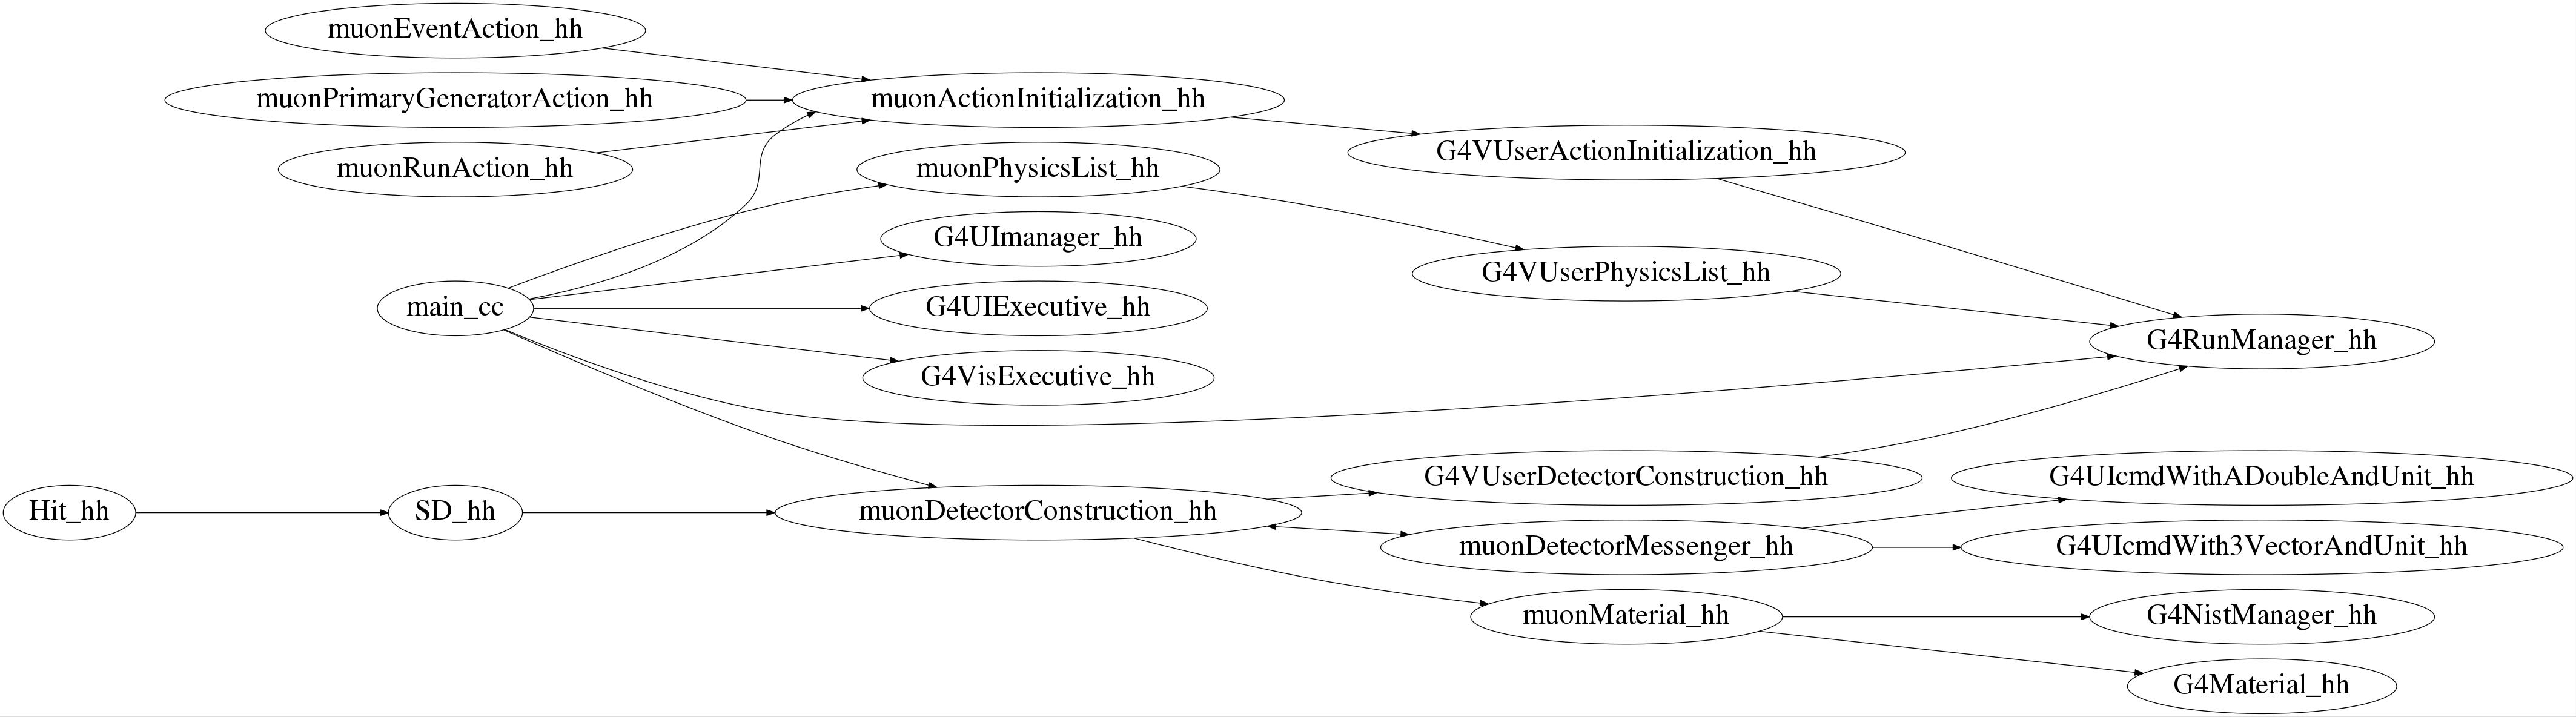
\includegraphics[width=120mm,height=40mm]{pic/main.jpg}
    \caption{程序的整体结构框图}
\end{figure}


程序运行由Geant4 的 G4RunManager 类控制,muonPhysicsList 类是控制粒子的物理过程,muonDetectorConstruction 是控制探测器几何信息,其中 muonMaterials是控制探测器的材料信息,muonDetectorMessenger 是用户交互控制探测器位置,尺寸信息。Action 类分别是控制初级粒子动力学信息的 muonPrimaryGeneratorAction 类和处理程序运行开始前和结束的一些操作的 muonRunAction,和击中信息的数字化,数据的输出的muonEventAction类。

\subsection{探测器几何}

如下图所示,两块探测器板都覆盖了1mm厚氧化铝的反射层,设置反射率为1,上底面没有覆盖反射层,所以探测器产生的光子会从上底面射出,上底面设置了聚丙烯的接受面,用于记录光子的达到时间以及光子的能量信息,探测器是一个高338.5mm,下底长143.5mm,上底长84mm,厚度为20mm,材料为蒽,分子式为C14H10的梯形结构。探测器折射率设置为1.3,反射层设置为1.76,光子在反射层的衰减长度为1m,在探测器的衰减长度为3m。探测器会输出缪子到达时间,缪子的位置信息和沉积的能量信息,可以通过缪子的位置信息判断缪子是否衰变。

\begin{figure}[h]
    \centering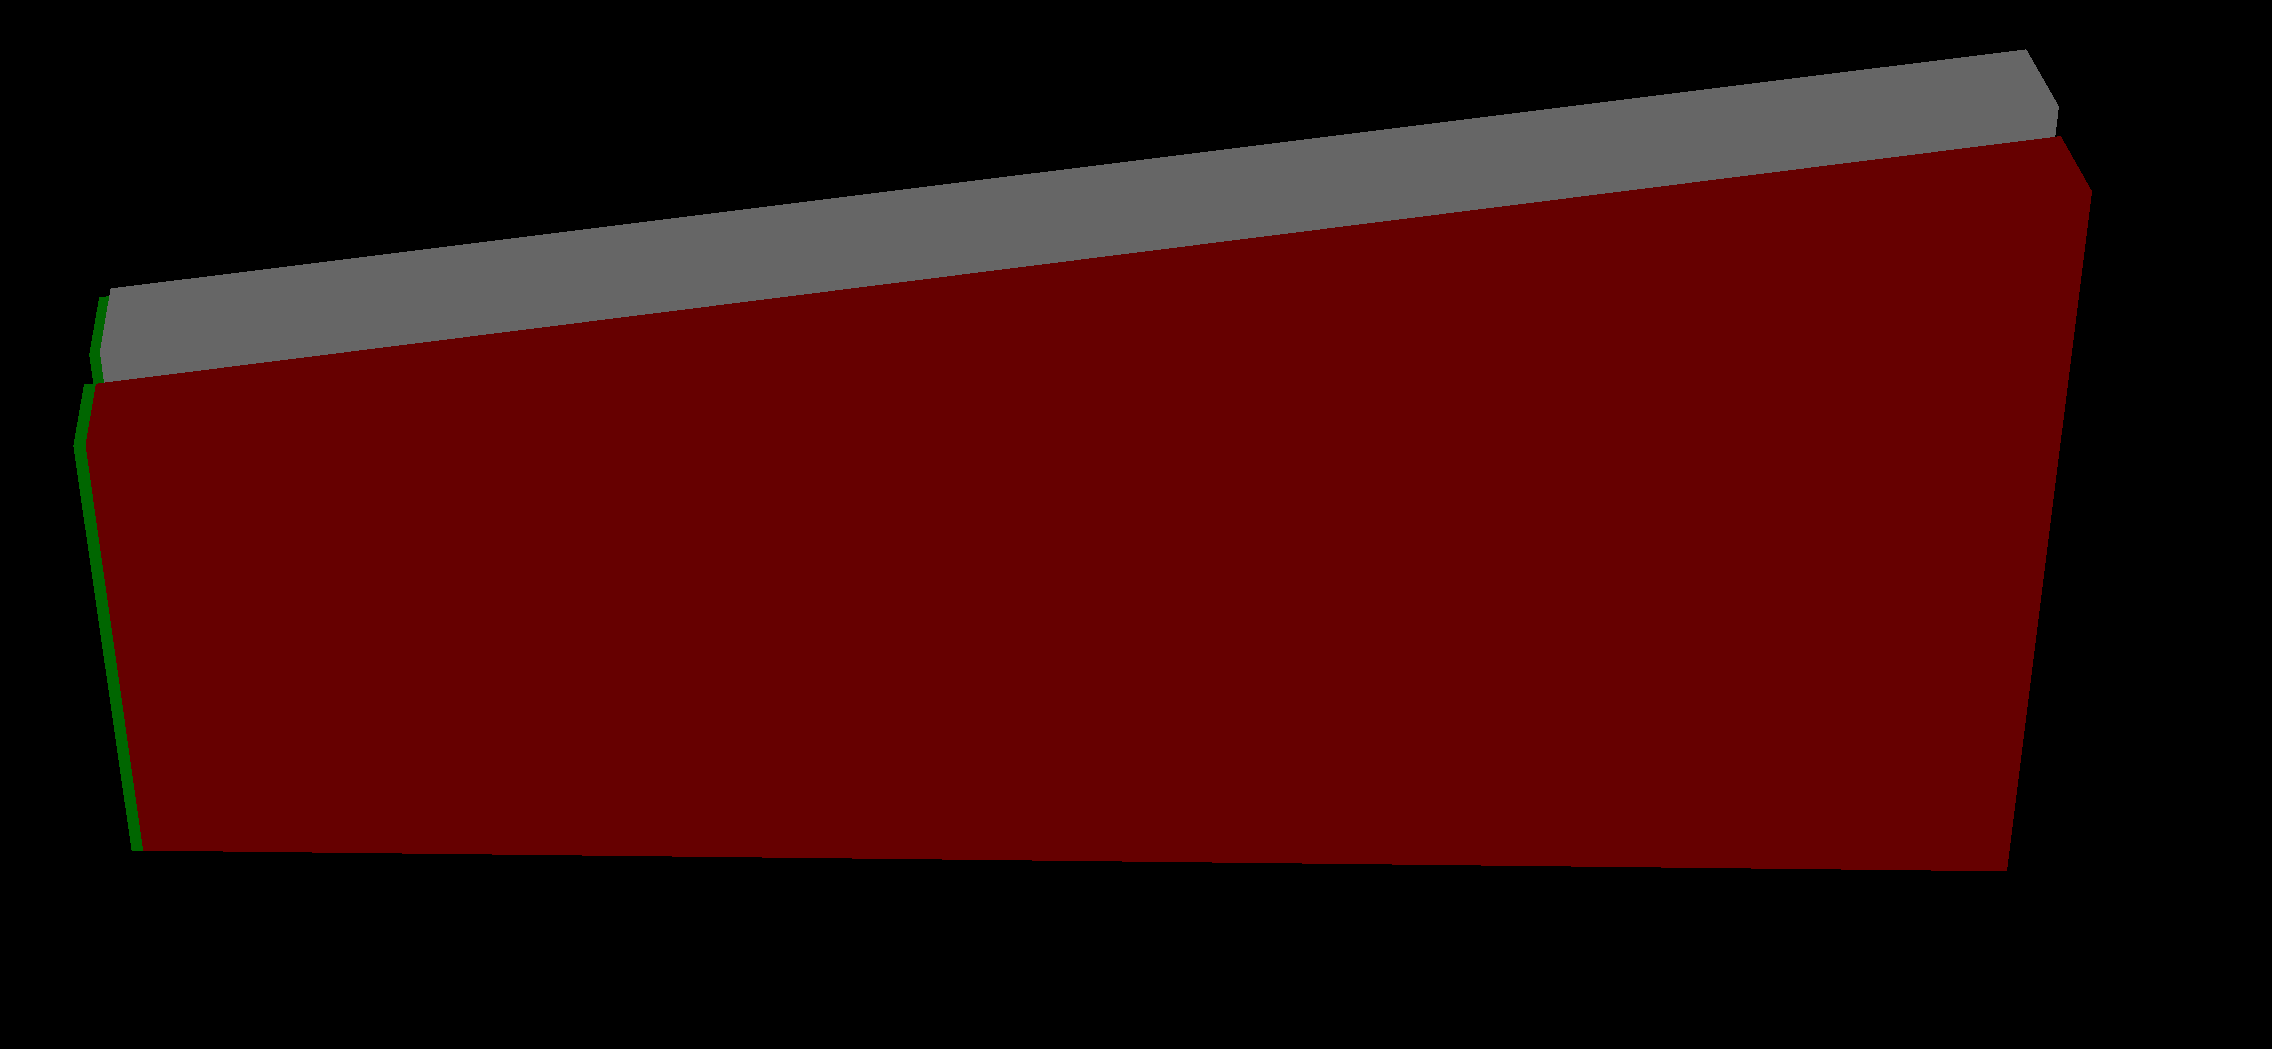
\includegraphics[width=120mm,height=40mm]{pic/muonde.png}
    \caption{探测器几何示意图}
\end{figure}

\subsection{探测器模拟的物理过程}

缪子从探测器上方 75mm 射入搭建的世界,世界材料为空气,所以经历了 muIoni , 其中 muIoni 会产生电子。\\

缪子在反射层 Al2O3 经历 Transportation 传播过程,损失大约 1.2 MeV 的能量, 以光子的形式被释放 Transportation 过程会放出少量光子. 缪子在塑料闪烁体中经历 muIoni 和Scintillation 闪烁过程\\

高能量缪子可直接从闪烁体中穿出, 并在径迹周围产生电子 ,以及荧光光子等次级粒子;一些较低能量 μ子在闪烁体中停止后,在塑料闪烁体中衰变放出anti\_nu\_e  nu\_mu  e-\\

G4Track Information: Particle = mu-, Track ID = 1,  Parent ID = 0\\
\begin{center}
\begin{tabular}{|c|c|c|c|c|c|}
 X(mm) & Y(mm) & Z(mm) & KinE(MeV)  & NextVolume & ProcName\\
 0    &  0      &  100  &  10   &       World &  initStep\\
 0.26 & -0.252  &  30.4 & 9.92  &        World &  muIoni\\
0.277  & -0.289 &   26 &  9.92  &   Al2O32 & Transportation\\
0.279 & -0.295  &  25.4 & 8.39  &     Al2O32  & muIoni\\
0.33 & -0.314  &    25 &  7.02 &    muondector2  & Transportation\\
0.714 &  -0.55 &  21.8 &  0    &    muondector2  & muIoni\\
0.714 & -0.55  &   21.8 &  0     & muondector2 & Scintillation

\end{tabular}
\end{center}

anti\_nu\_e nu\_mu经历Transportation\\

G4Track Information:   Particle = nu\_mu,   Track ID = 21,   Parent ID = 1\\

\begin{center}
\begin{tabular}{|c|c|c|c|c|c|}
X(mm) & Y(mm) & Z(mm) & KinE(MeV)  & NextVolume & ProcName\\
0.714 & -0.55 &  21.8 & 30.7 &   muondector2 & initStep\\
-19.9 &   -51.2  &    100   &   30.7  & OutOfWorld  & Transportation

\end{tabular}
\end{center}

G4Track Information:   Particle =  anti\_nu\_e,   Track ID = 20,   Parent ID = 1\\

\begin{center}
\begin{tabular}{|c|c|c|c|c|c|}
X(mm) & Y(mm) & Z(mm) & KinE(MeV)  & NextVolume & ProcName\\
0.714 & -0.55 &  21.8 & 24.4 &   muondector2 & initStep\\
-24.6 &   45.6  &    100   &   24.4  & OutOfWorld  & Transportation

\end{tabular}
\end{center}

电子在塑料闪烁体中经历 eBrem 和 Cerenkov 释放大量光子,同时经过 eIoni 释放低能电子和 gamma 光子,最后经历Scintillation\\

电子在空气中也是经历eIoni 和Scintillation 闪烁过程 eIonic 过程会放出低能电子。\\

G4Track Information:   Particle = e-,   Track ID = 19,   Parent ID = 1\\

\begin{center}
\begin{tabular}{|c|c|c|c|c|c|}

X(mm)  &  Y(mm)  &  Z(mm) & KinE(MeV)  &  NextVolume & ProcName\\
0.714  &  -0.55   &  21.8 &    50  &    muondector2 & initStep\\
1.44  &  -0.158    &   19     &  47.7   & muondector2 & eBrem\\
3.74   &   1.76  &   8.21   &   45.5     &  muondector2 & Cerenkov\\
4.37    & 2.3 &  5  &  44.8   &     Al2O32  & Transportation\\
4.53  &   2.37  &  4 & 44.3  &     World & Transportation\\
5.77  &  3.07  & -4.88   &  38   &  Al2O31 & eBrem (已经到达了)\\
5.85  & 3.08 & -5.55  &   34.3   &  muondector1 & eIoni(已经到达了 0.0896MeV)\\
\end{tabular}
\end{center}


G4Track Information:   Particle = e-,   Track ID = 577,   Parent ID = 19\\

\begin{center}
\begin{tabular}{|c|c|c|c|c|c|}
X(mm)  &  Y(mm)  &  Z(mm) & KinE(MeV)  &  NextVolume & ProcName\\
5.85  & 3.08  &  -5.55    &  3.55    & muondector1  & initStep\\
11.7  &  -1.3 & -14.7    &   0.448    & muondector1 & eIoni\\
12 & -1.15 & -15.1   &    0   &  muondector1  & Cerenkov\\
 12  & -1.15  & -15.1    &   0     &  muondector1  & Scintillation

\end{tabular}
\end{center}


\section{缪子探测器模拟初步结果分析}
\subsection{探测器优化}

我们利用该程序测试了厚度都是为20mm的两个探测器的性能,将它们相距10mm,其中包括两个反射层的厚度,入射粒子为$\mu^-$,能量从0.01GeV/10MeV到0.069GeV/69MeV,间隔为1MeV,每个缪子能量都运行了1000个事例。然后计算缪子的穿透距离和沉积能量以及单位距离的沉积能量的平均值和方差。\\

\begin{figure}[H]
    \centering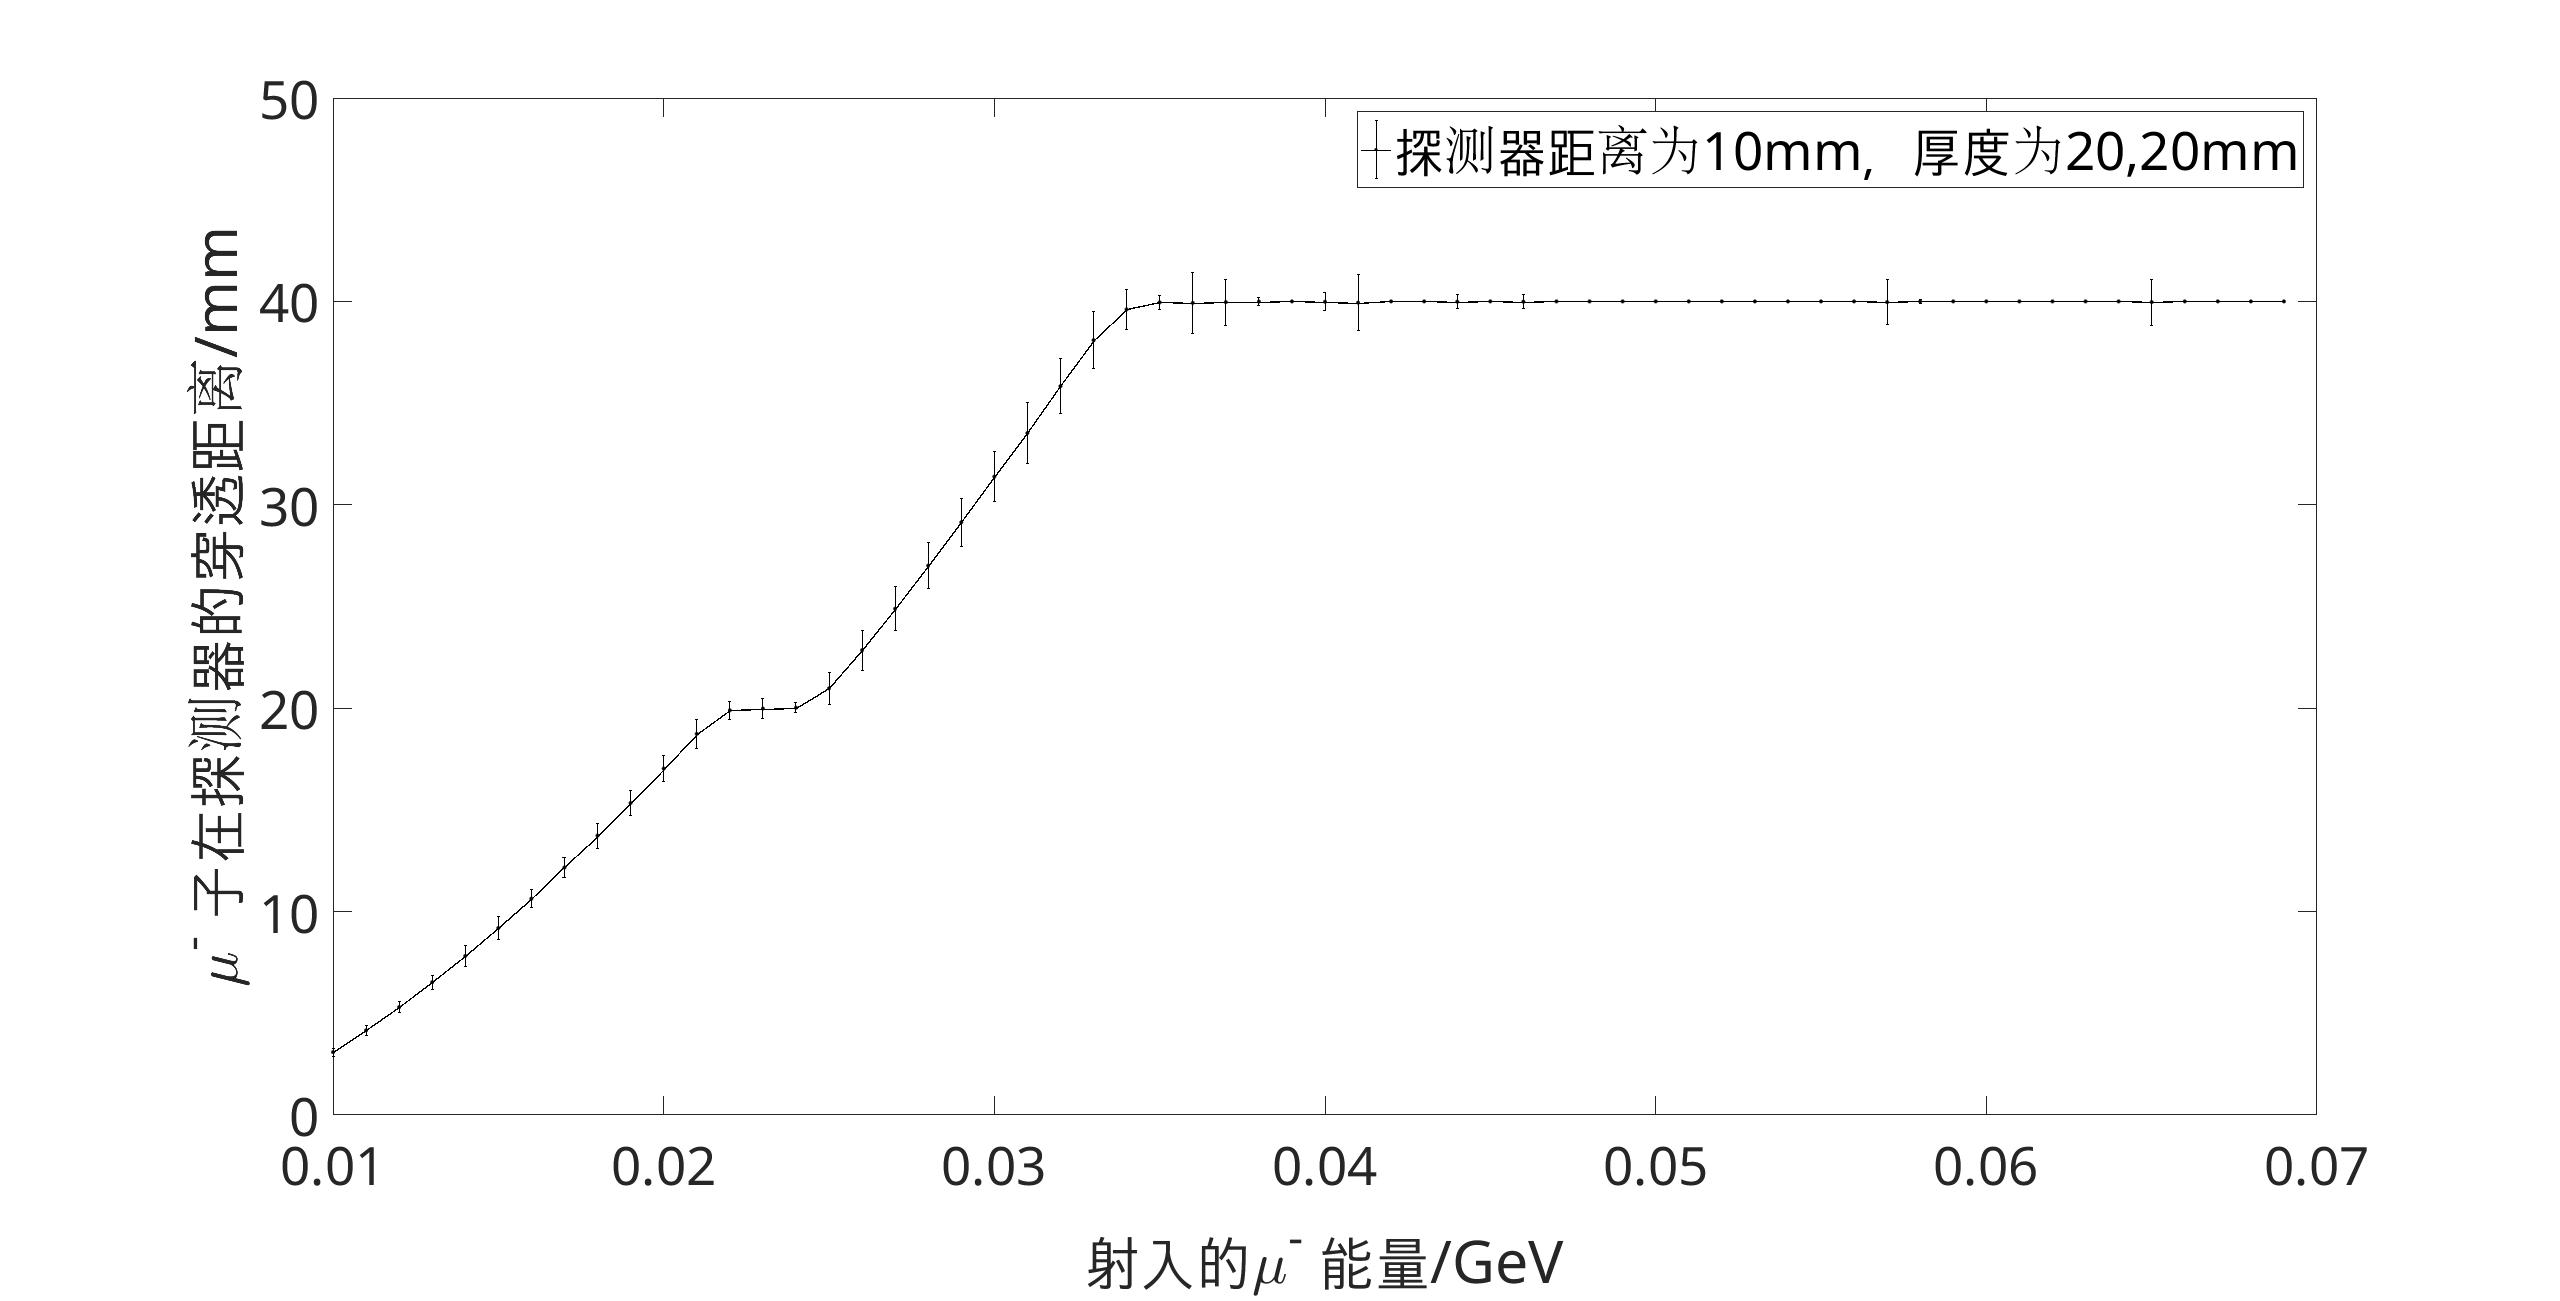
\includegraphics[width=100mm,height=50mm]{pic/de_distant_dis_10_se_20.jpg}
    \caption{缪子在探测器中穿透距离随着入射的缪子能量的变化曲线}\label{di1020}
\end{figure}


如图\ref{di1020}所示,该图表示缪子在探测器中穿透距离随着入射的缪子能量的变化,由图可以看出第一个上升曲线的穿透距离小于20mm,说明缪子在第一个探测器中衰变,说明极低能的缪子会在第一个探测器中衰变,然后经过一个平台,到达第二个探测器中。之所以出现平台是因为我们只统计了缪子在探测器中运行距离,中间平台说明缪子需要耗费一定的能量才能到达第二个探测器中。需要说明的一点是为什么穿透距离到达了探测器的总厚度的时候,还会有方差不为0,这就表明了高能量的缪子在探测器衰变的几率已经很小了,已经跑出探测器了。但是高能量的缪子还是有可能在探测器中衰变,一旦衰变,穿透距离不等于探测器厚度,那么平均值也就比厚度小,这样绝大部分的穿透距离为厚度,这样方差就不为0了,由此造成的方差也可能会很大。\\


\begin{figure}[H]
    \centering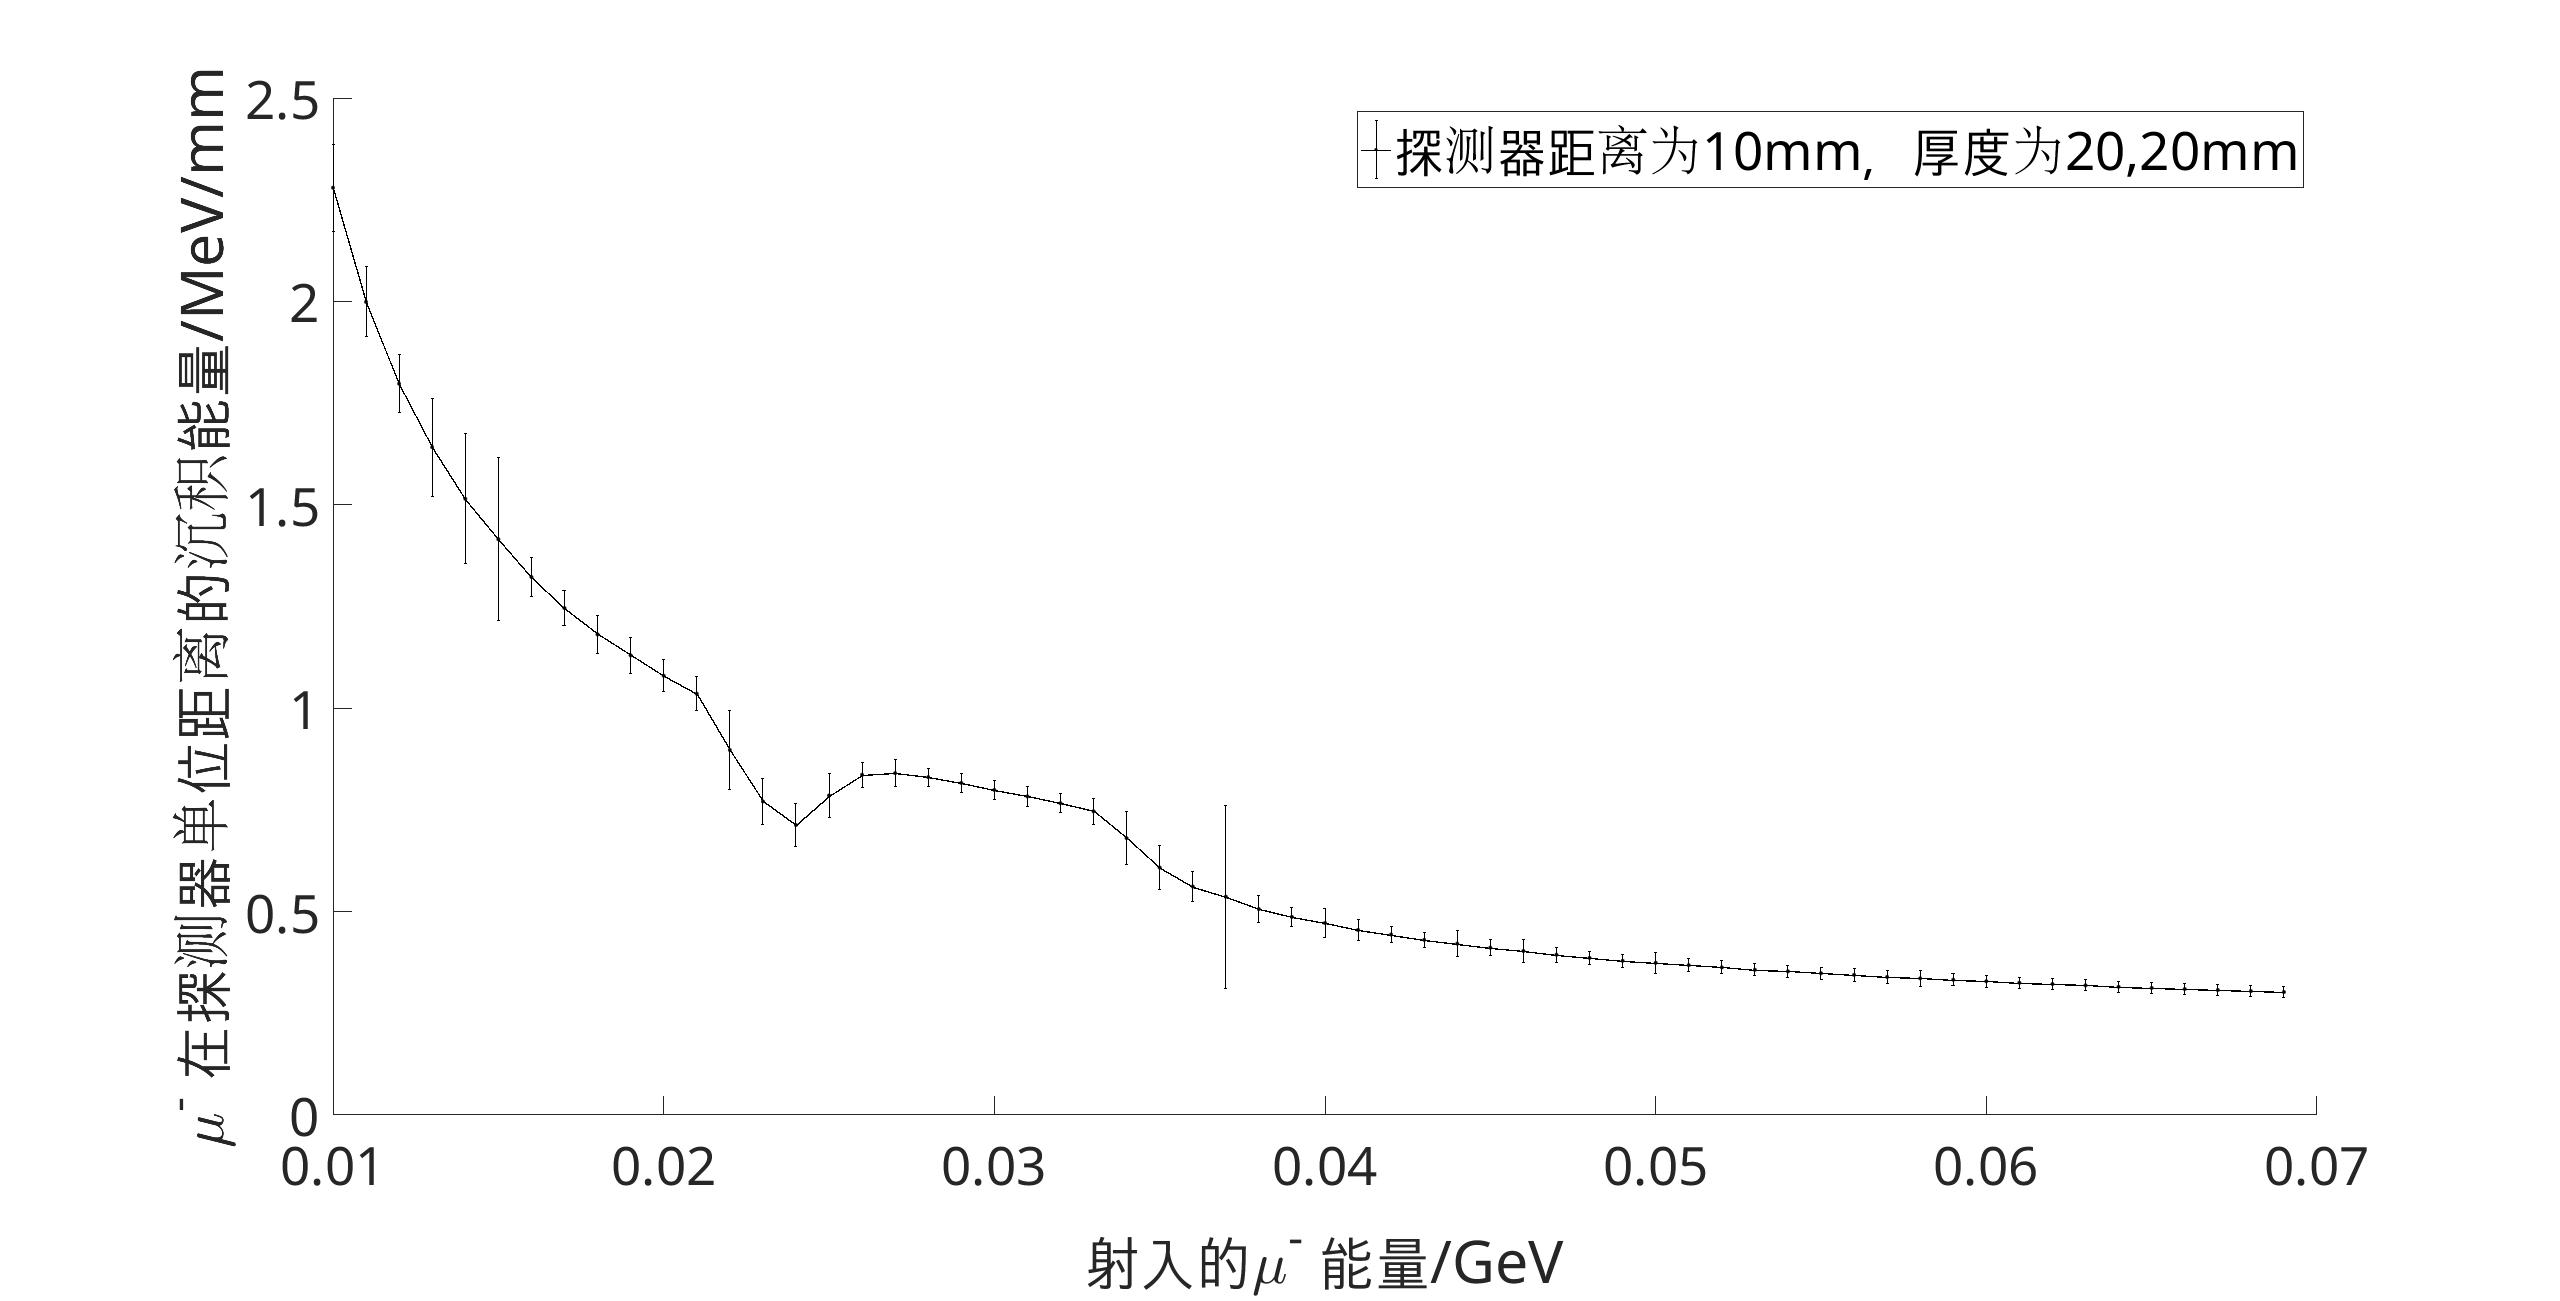
\includegraphics[width=100mm,height=50mm]{pic/de_en_di_dis_10_se_20.jpg}
    \caption{缪子在探测器中单位距离沉积能量随着入射的缪子能量的变化曲线}\label{en_di1020}
\end{figure}


如图\ref{en_di1020}所示,该图表示缪子在探测器中单位距离沉积能量随着入射的缪子能量的变化,由图我们可以看出单位距离沉积能量基本是随着入射的缪子能量指数下降,一开始由于能量不够,基本所有能量都会损失到探测器中,所以缪子速度就慢慢下降,考虑相对论的效应就会下降,(这里应该是有一个物理过程跟速度有关让它会多损失能量),所以在缪子足够大的能量时,比如在分别可以通过第一个探测器和第二个探测器的时候,单位距离沉积能量就有一个小的快速下降的趋势。\\

\begin{figure}[H]
    \centering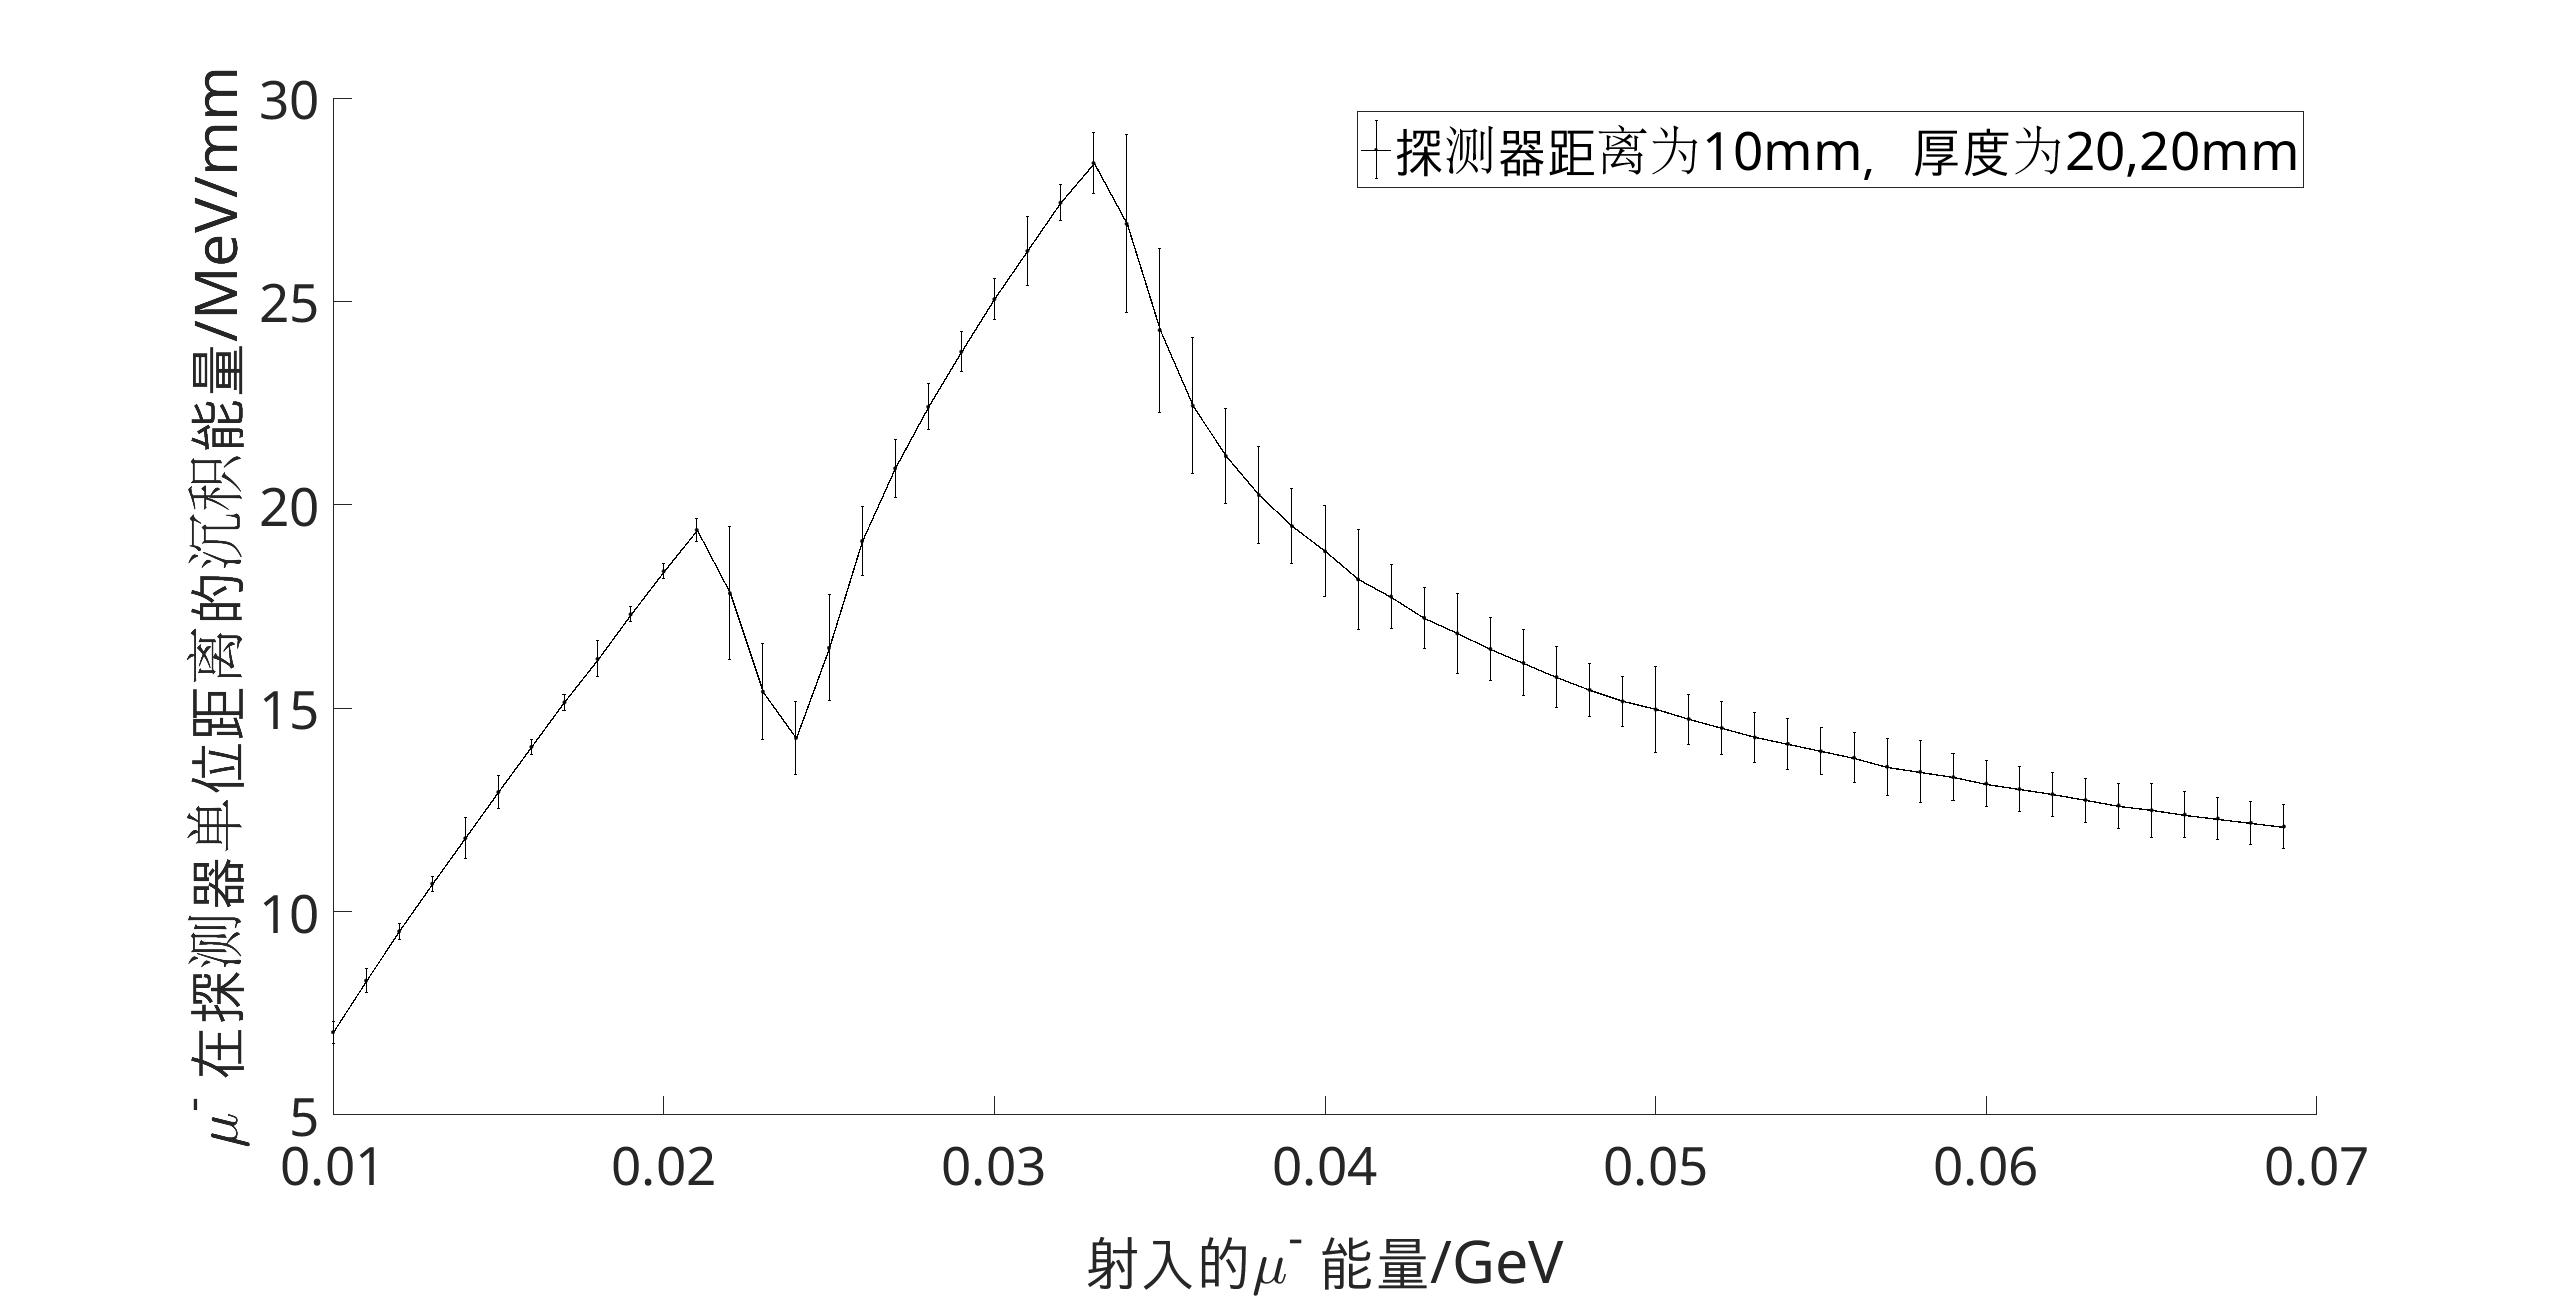
\includegraphics[width=100mm,height=50mm]{pic/de_en_dis_10_se_20.jpg}
    \caption{缪子在探测器中沉积能量随着入射的缪子能量的变化曲线}\label{en1020}
\end{figure}

如图\ref{en1020}所示,该图表示缪子在探测器中沉积能量随着入射的缪子能量的变化,由图,可以知道穿透第一个探测器和第二个探测器大概需要多少能量,并且伴随穿透探测器有下降趋势的原因也是由于单位距离沉积能量下降的原因。

\subsubsection{探测器厚度的影响}

接着我们调整了第二个探测器的厚度分别为10mm,15mm,25mm,30mm,35mm,40mm,60mm,图\ref{fig:di}表明随着第二个探测器厚度增长,穿透距离也增大,我们读取达到稳定点的入射缪子能量做线性分析,得到下面参数,如图\ref{fig:di_linear}所示:\\

\begin{figure}[h]
\centering
    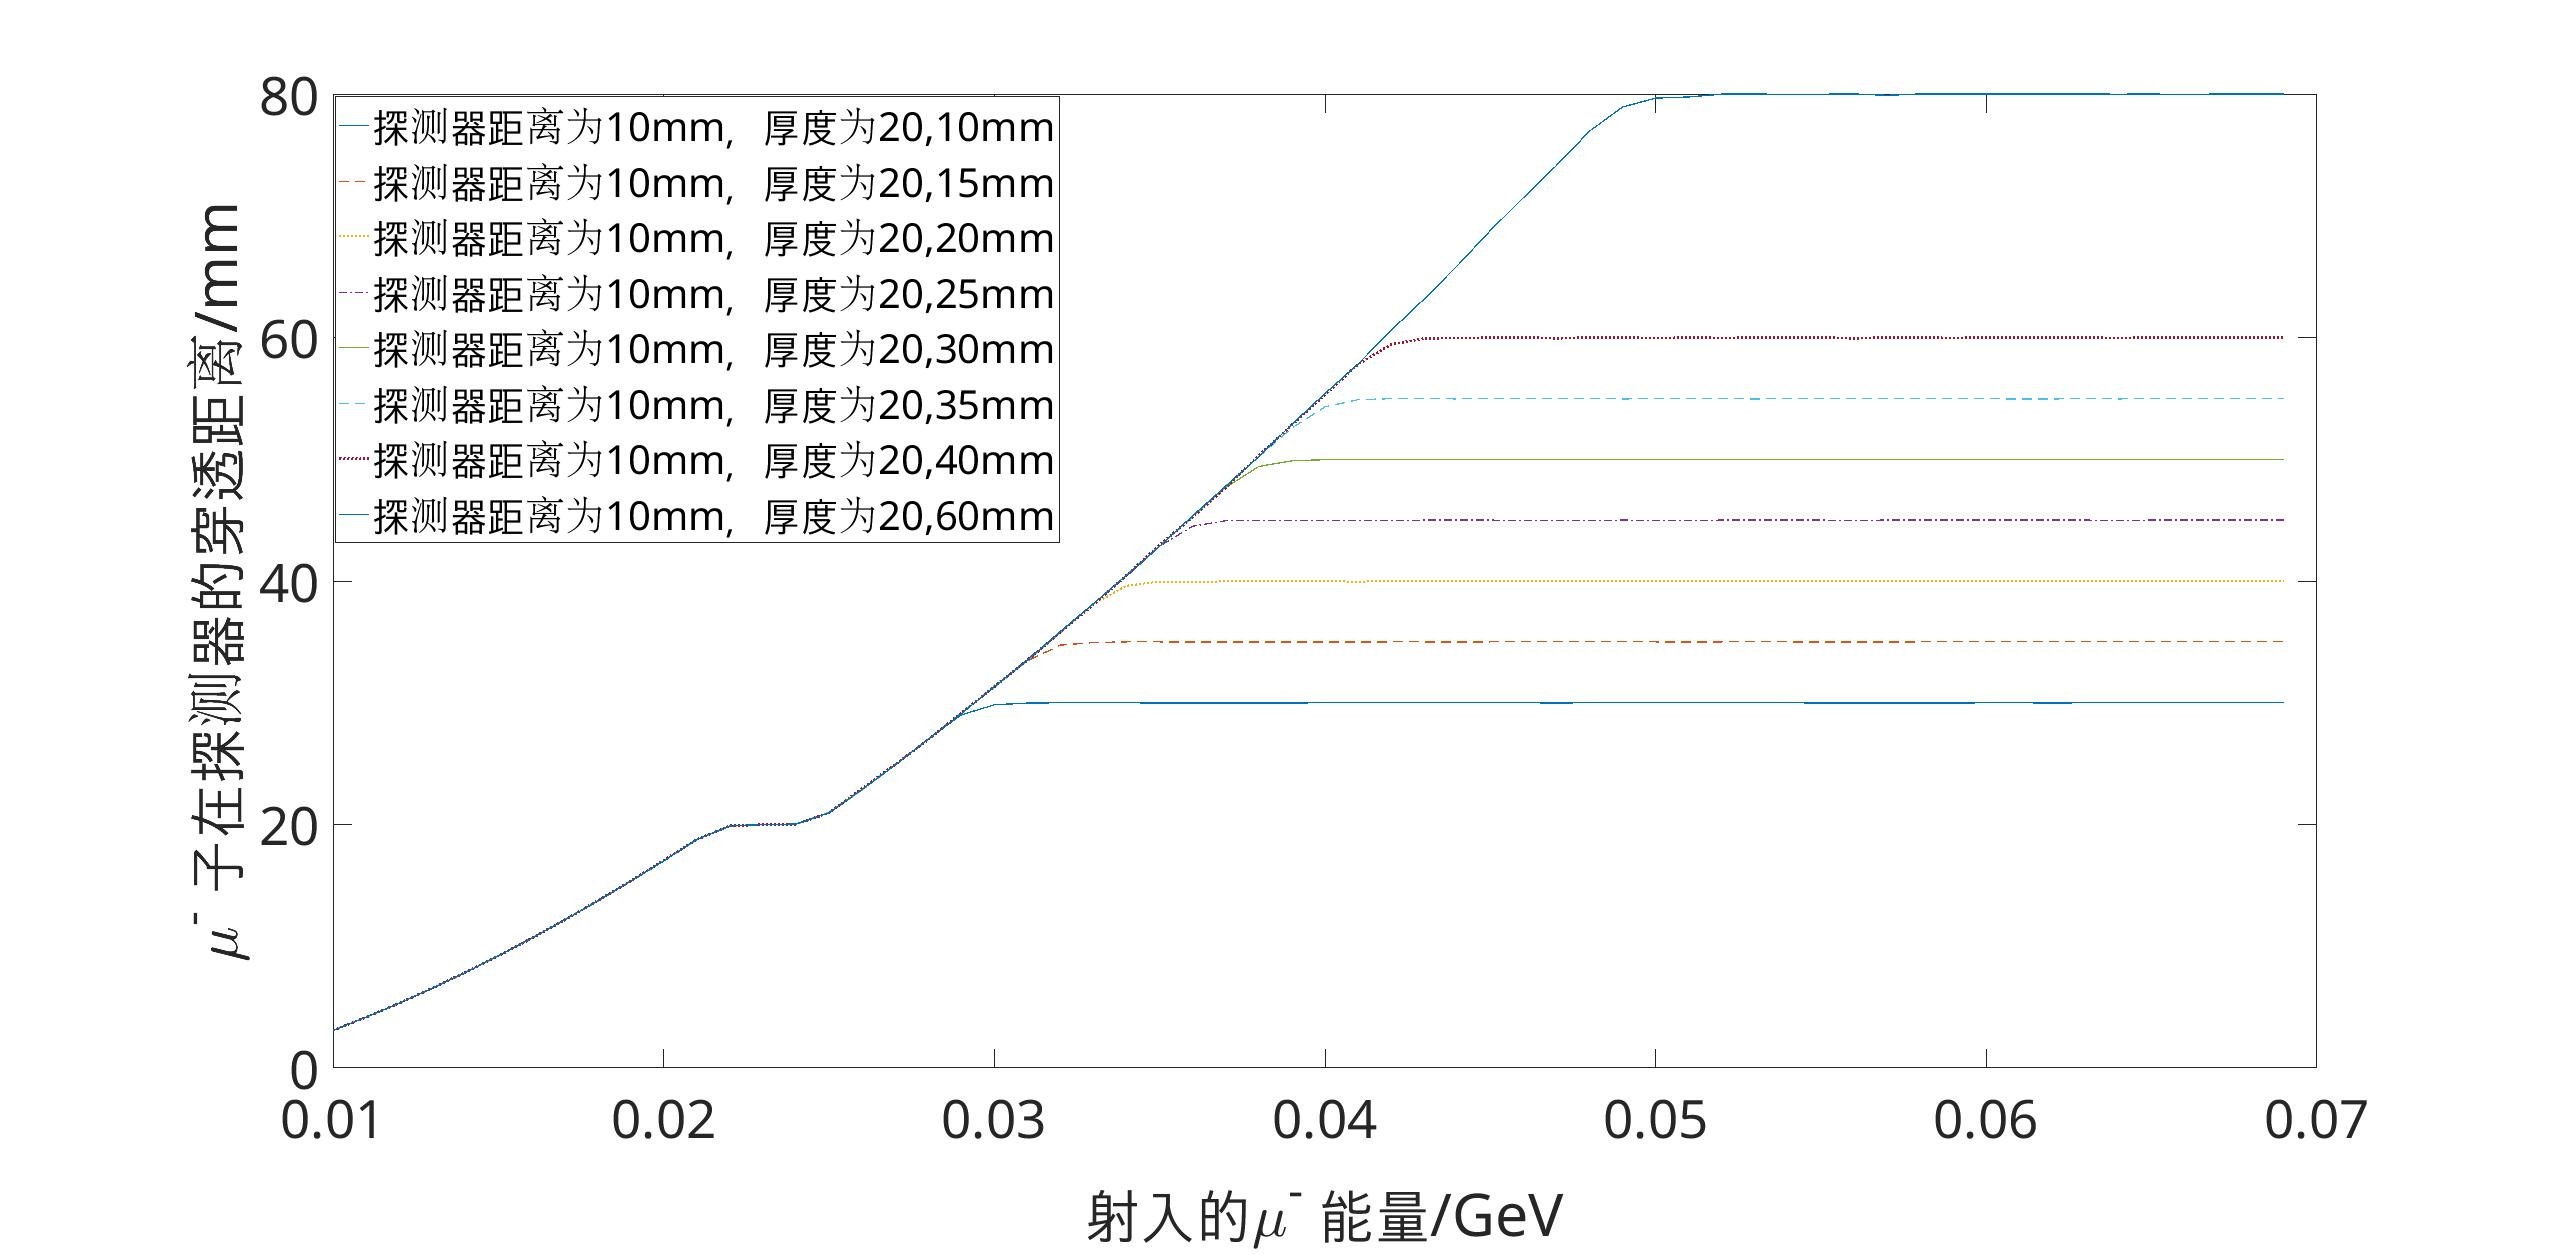
\includegraphics[width=120mm,height=60mm]{pic/dis.jpg}
    \caption{厚度不同的穿透曲线}\label{fig:di}
    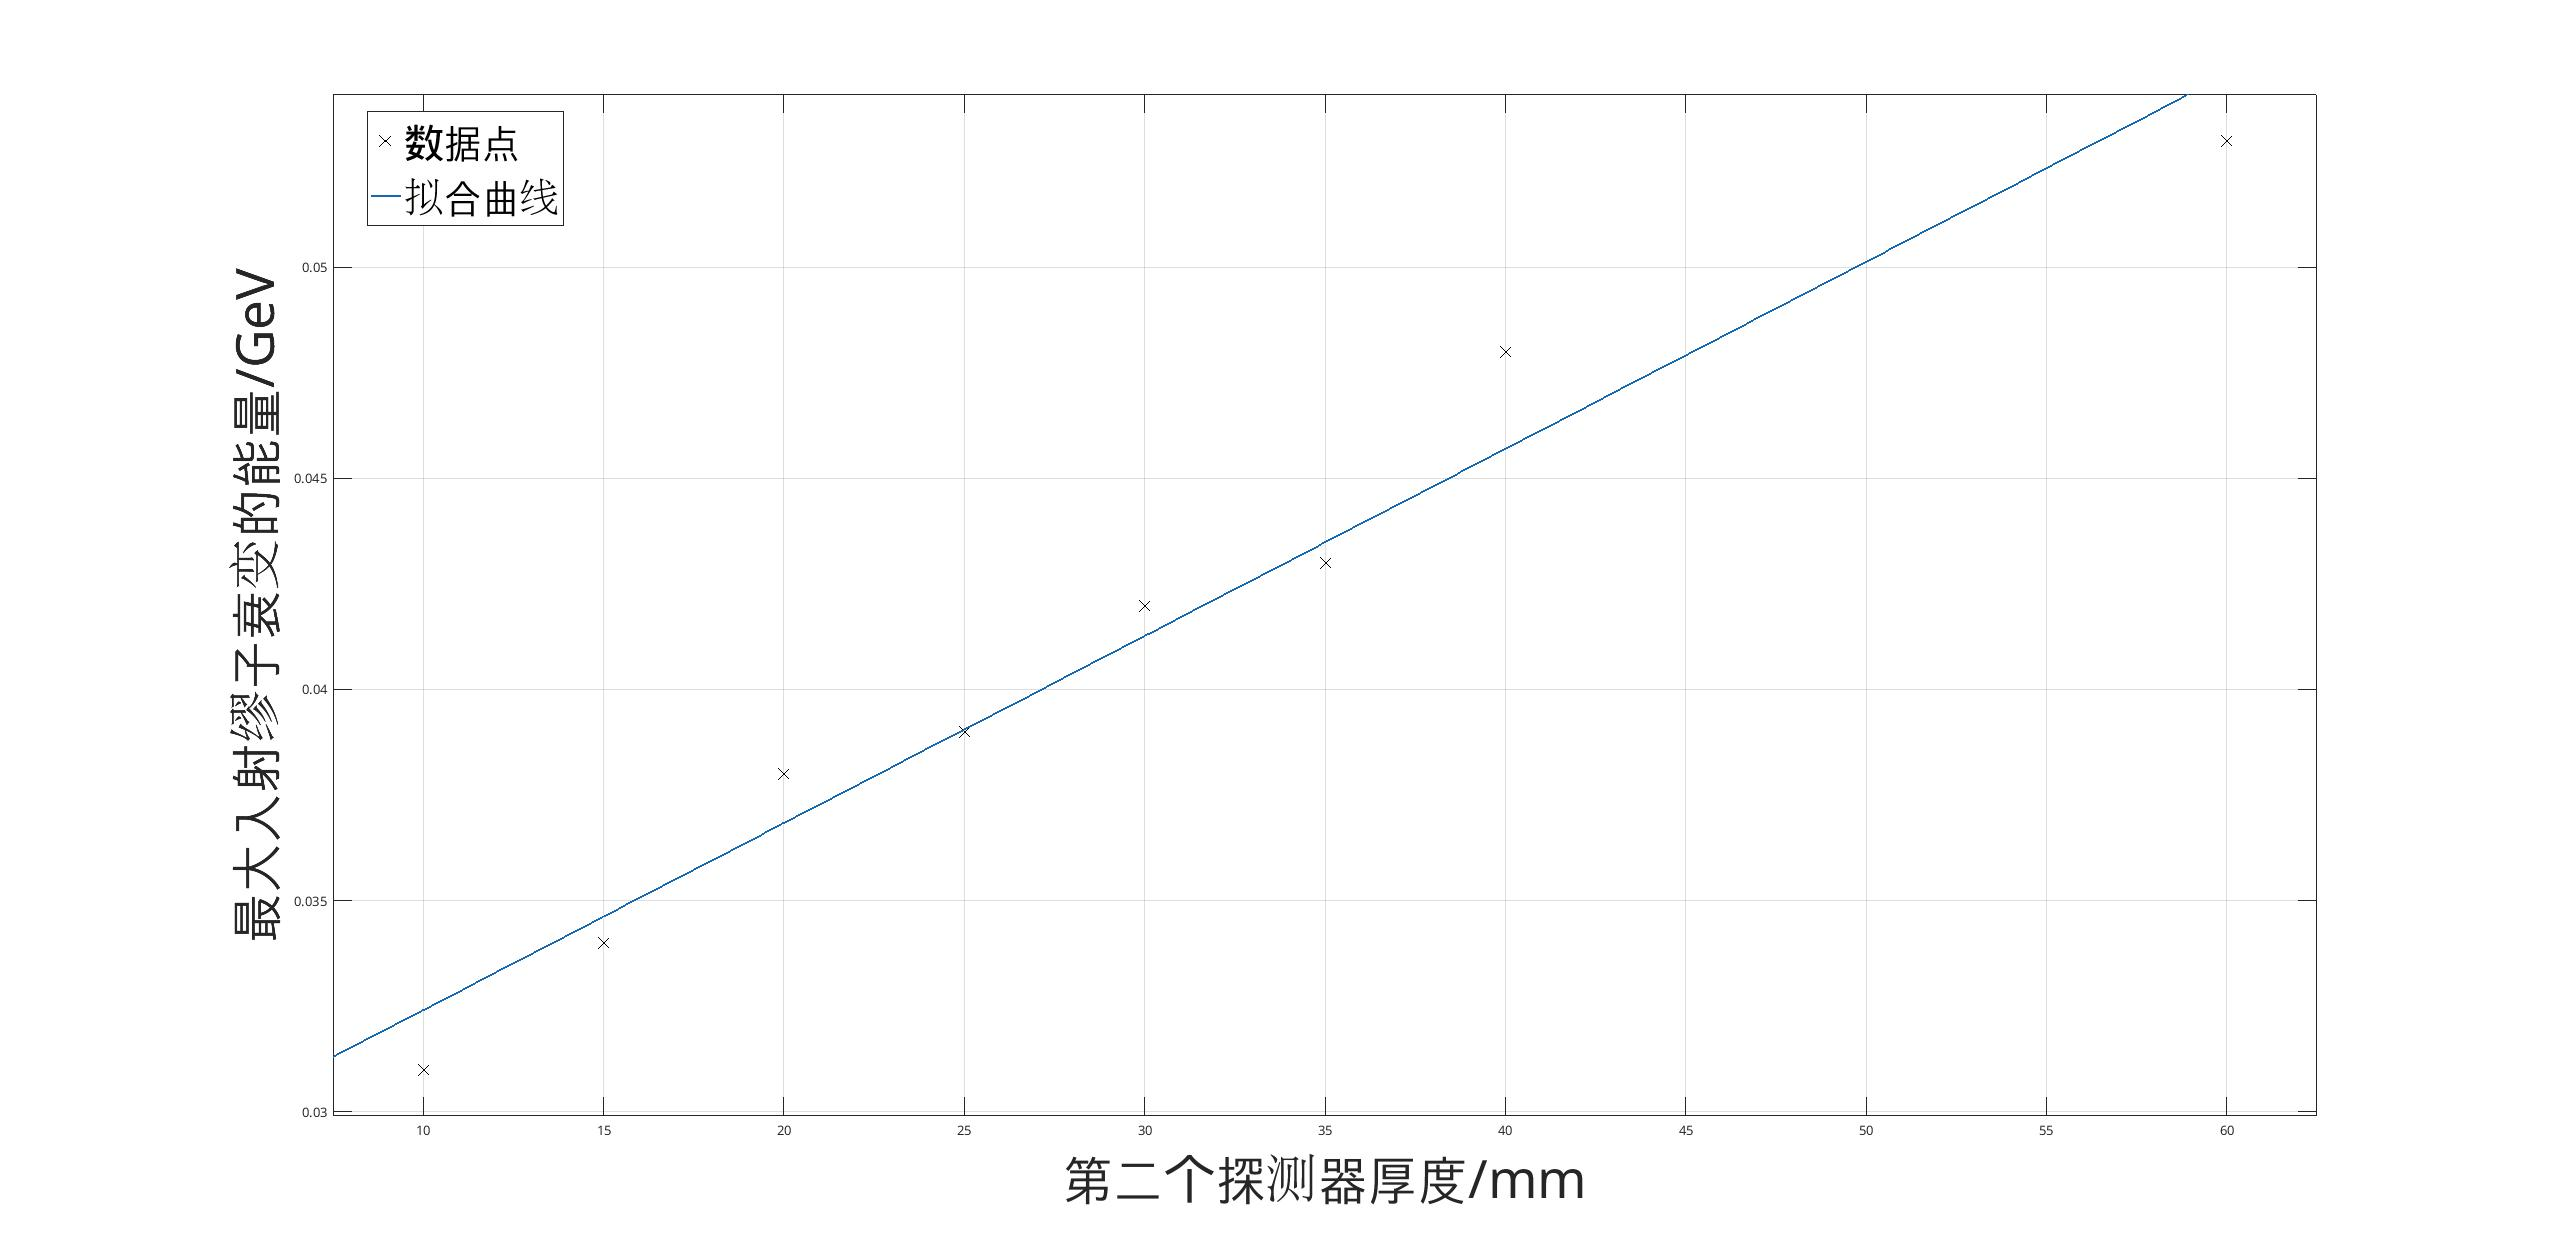
\includegraphics[width=80mm,height=40mm]{pic/quxian.jpg}
    \caption{最大入射缪子衰变的能量和探测器厚度的关系}\label{fig:di_linear}
\end{figure}


拟合公式为 $k\times x + b$,其中$k = 0.000443,\ b= 0.02799$,R-square:0.9961\\


由这些参数可以知道在第二个探测器最大入射缪子衰变的能量和探测器厚度基本是线性关系,所以我们可以调控第一个探测器的厚度来控制缪子在第二个探测器衰变的最小能量,通过调控第二个探测器的厚度来控制缪子在第二个探测器衰变的最大能量,考虑探测器的造假,我们可以让该能量区间对应缪子达到地球表面能量几率最大并且最经济的区间。\\

\begin{figure}[H]
\centering
    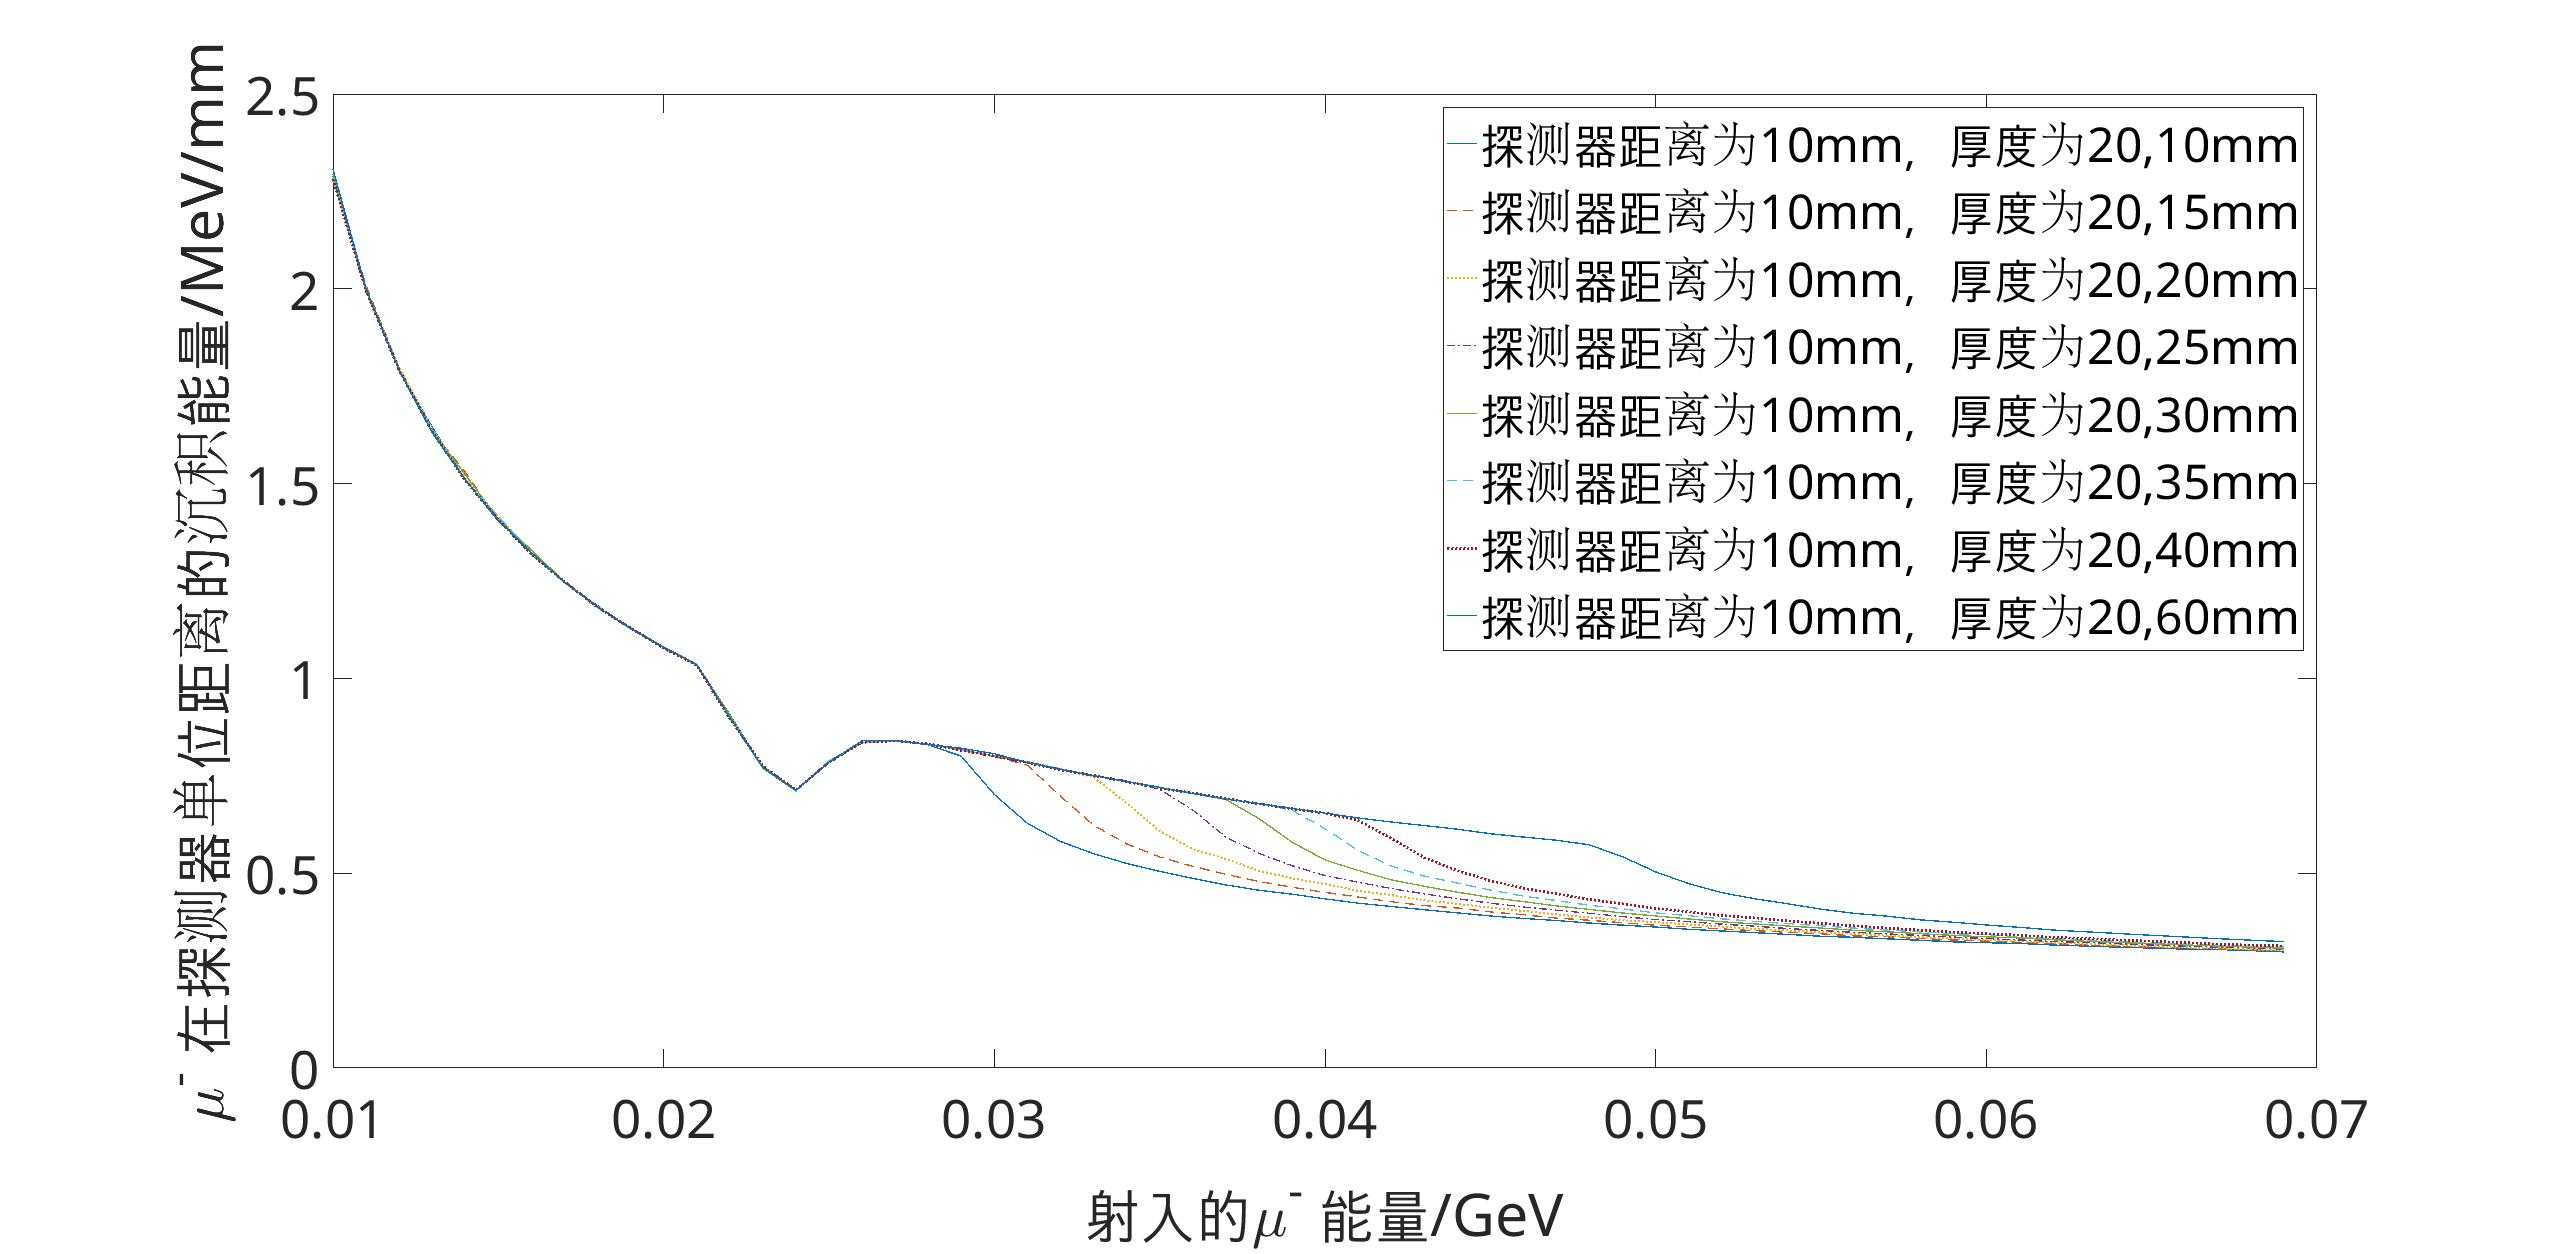
\includegraphics[width=120mm,height=60mm]{pic/en_dis.jpg}
    \caption{厚度不同单位距离沉积能量的曲线}
\end{figure}


单位距离沉积能量的图 不知道可以得出什么结论


\subsubsection{探测器的距离的影响}

接下来我们分析探测器的距离对探测器性能的影响,由下三个图知道距离对探测器的影响可以忽略不计,但是为了防止其他粒子从中间间隔入射,可以让距离变小。\\

\begin{figure}[H]
\centering
    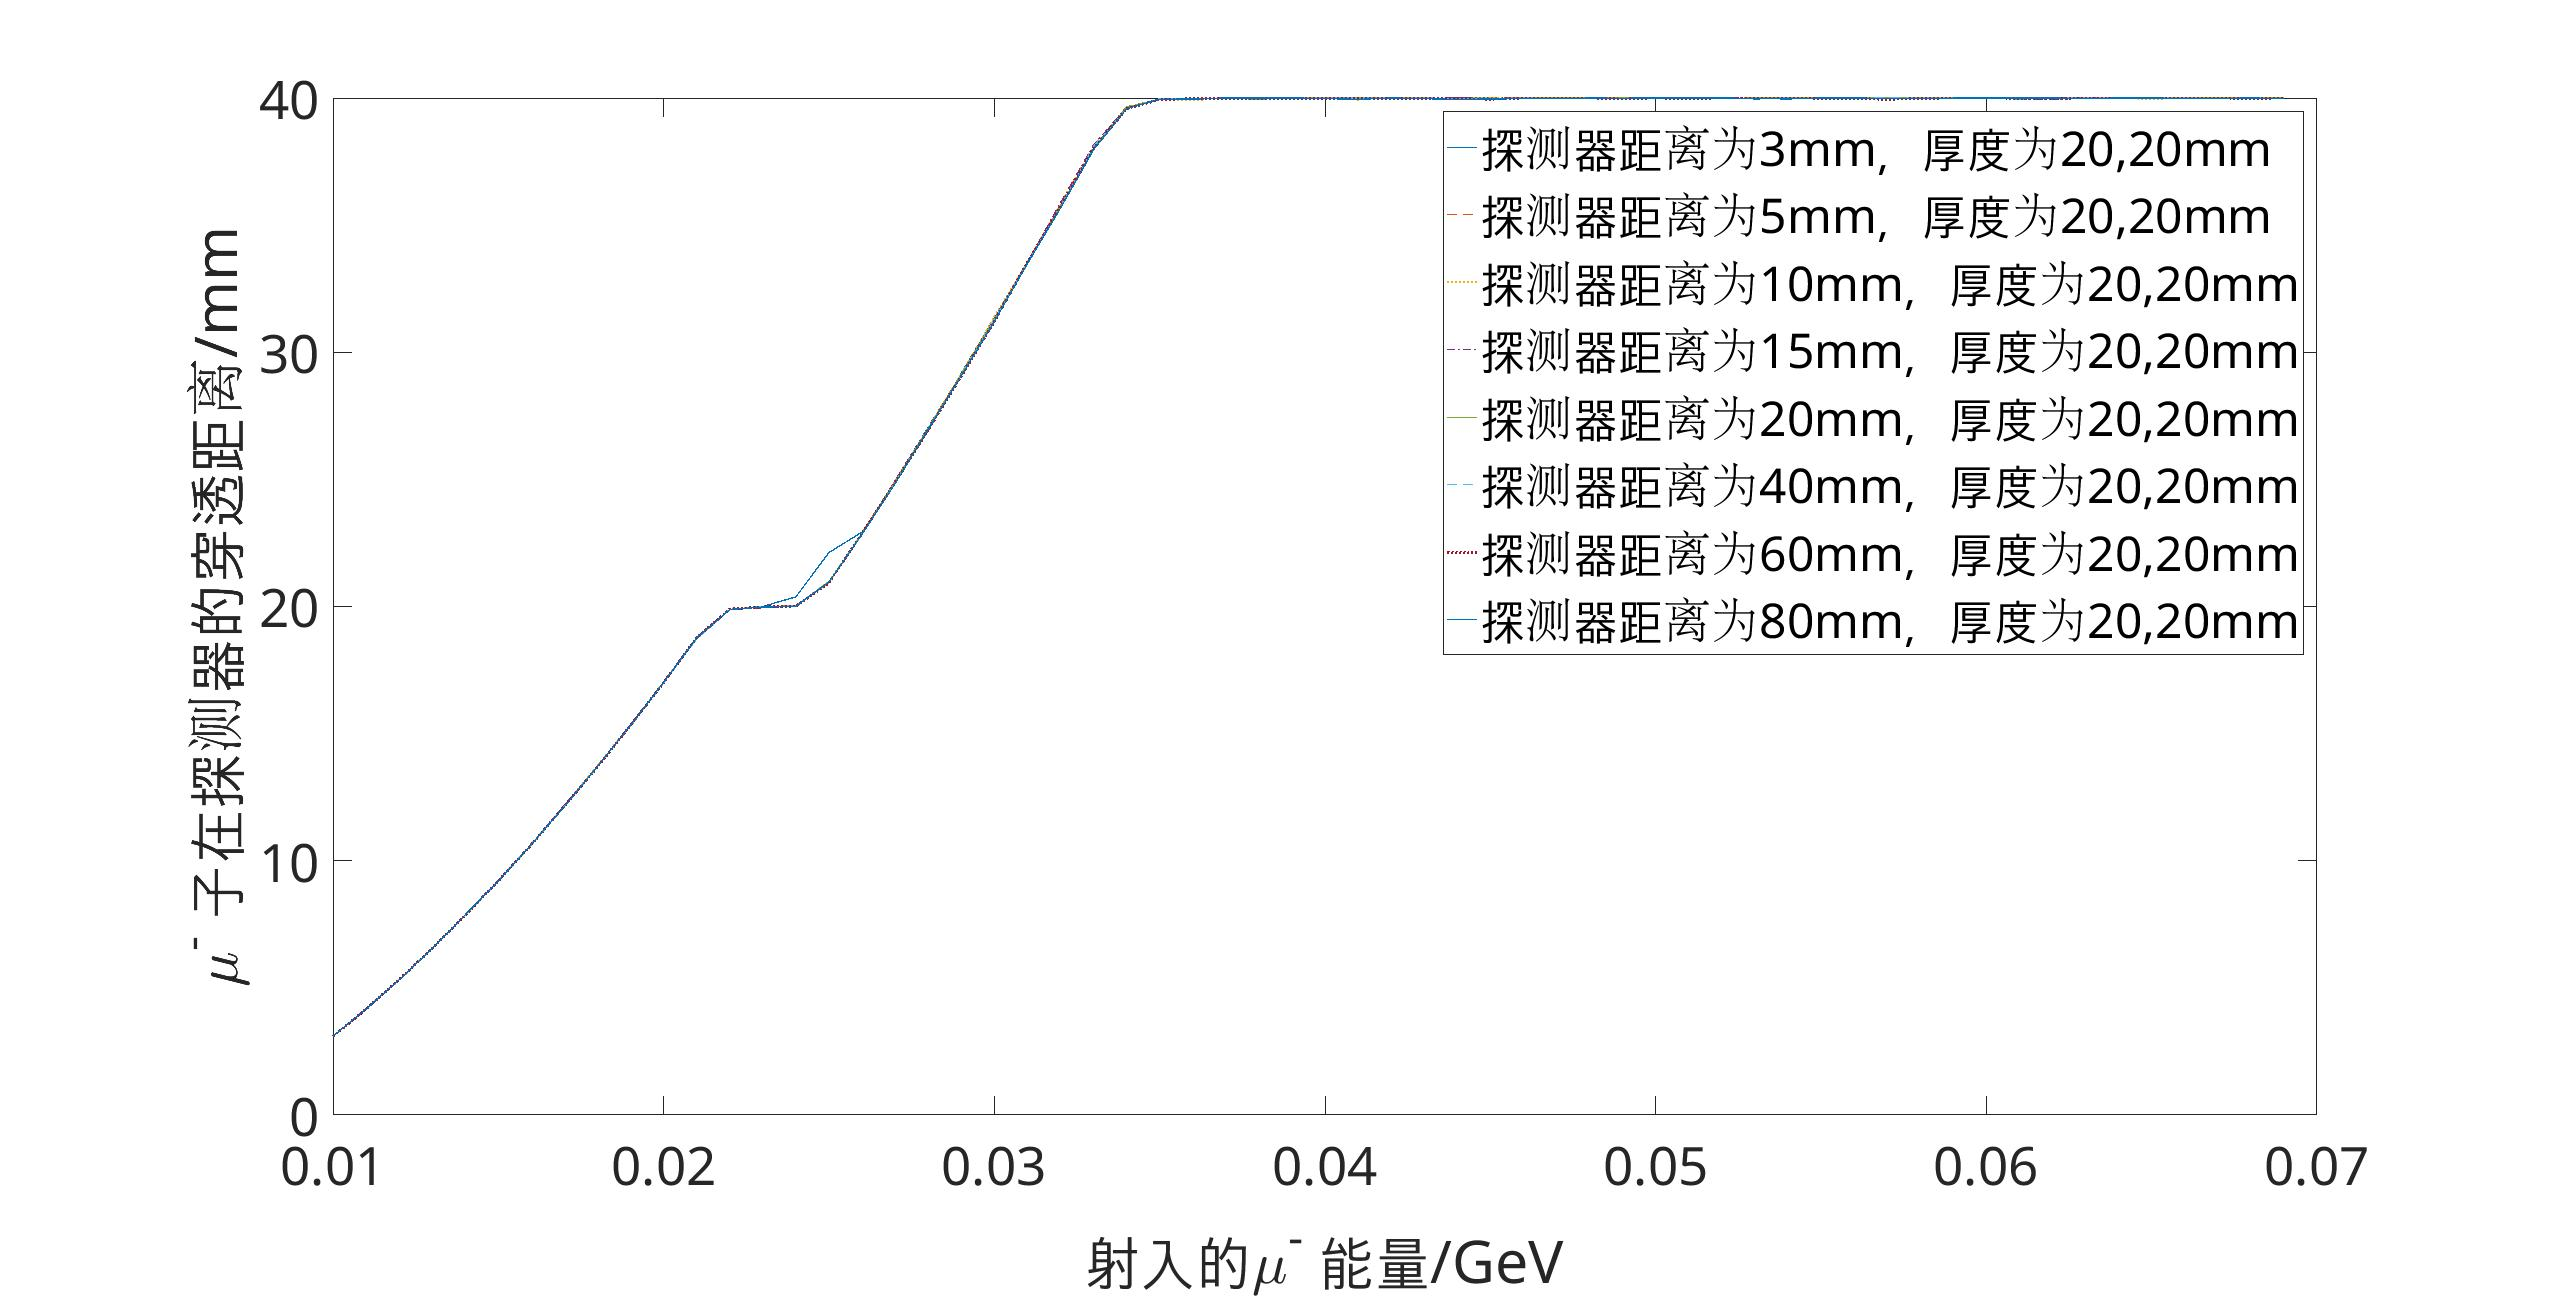
\includegraphics[width=120mm,height=60mm]{pic/dis_all.jpg}
    \caption{距离不同的穿透曲线}
    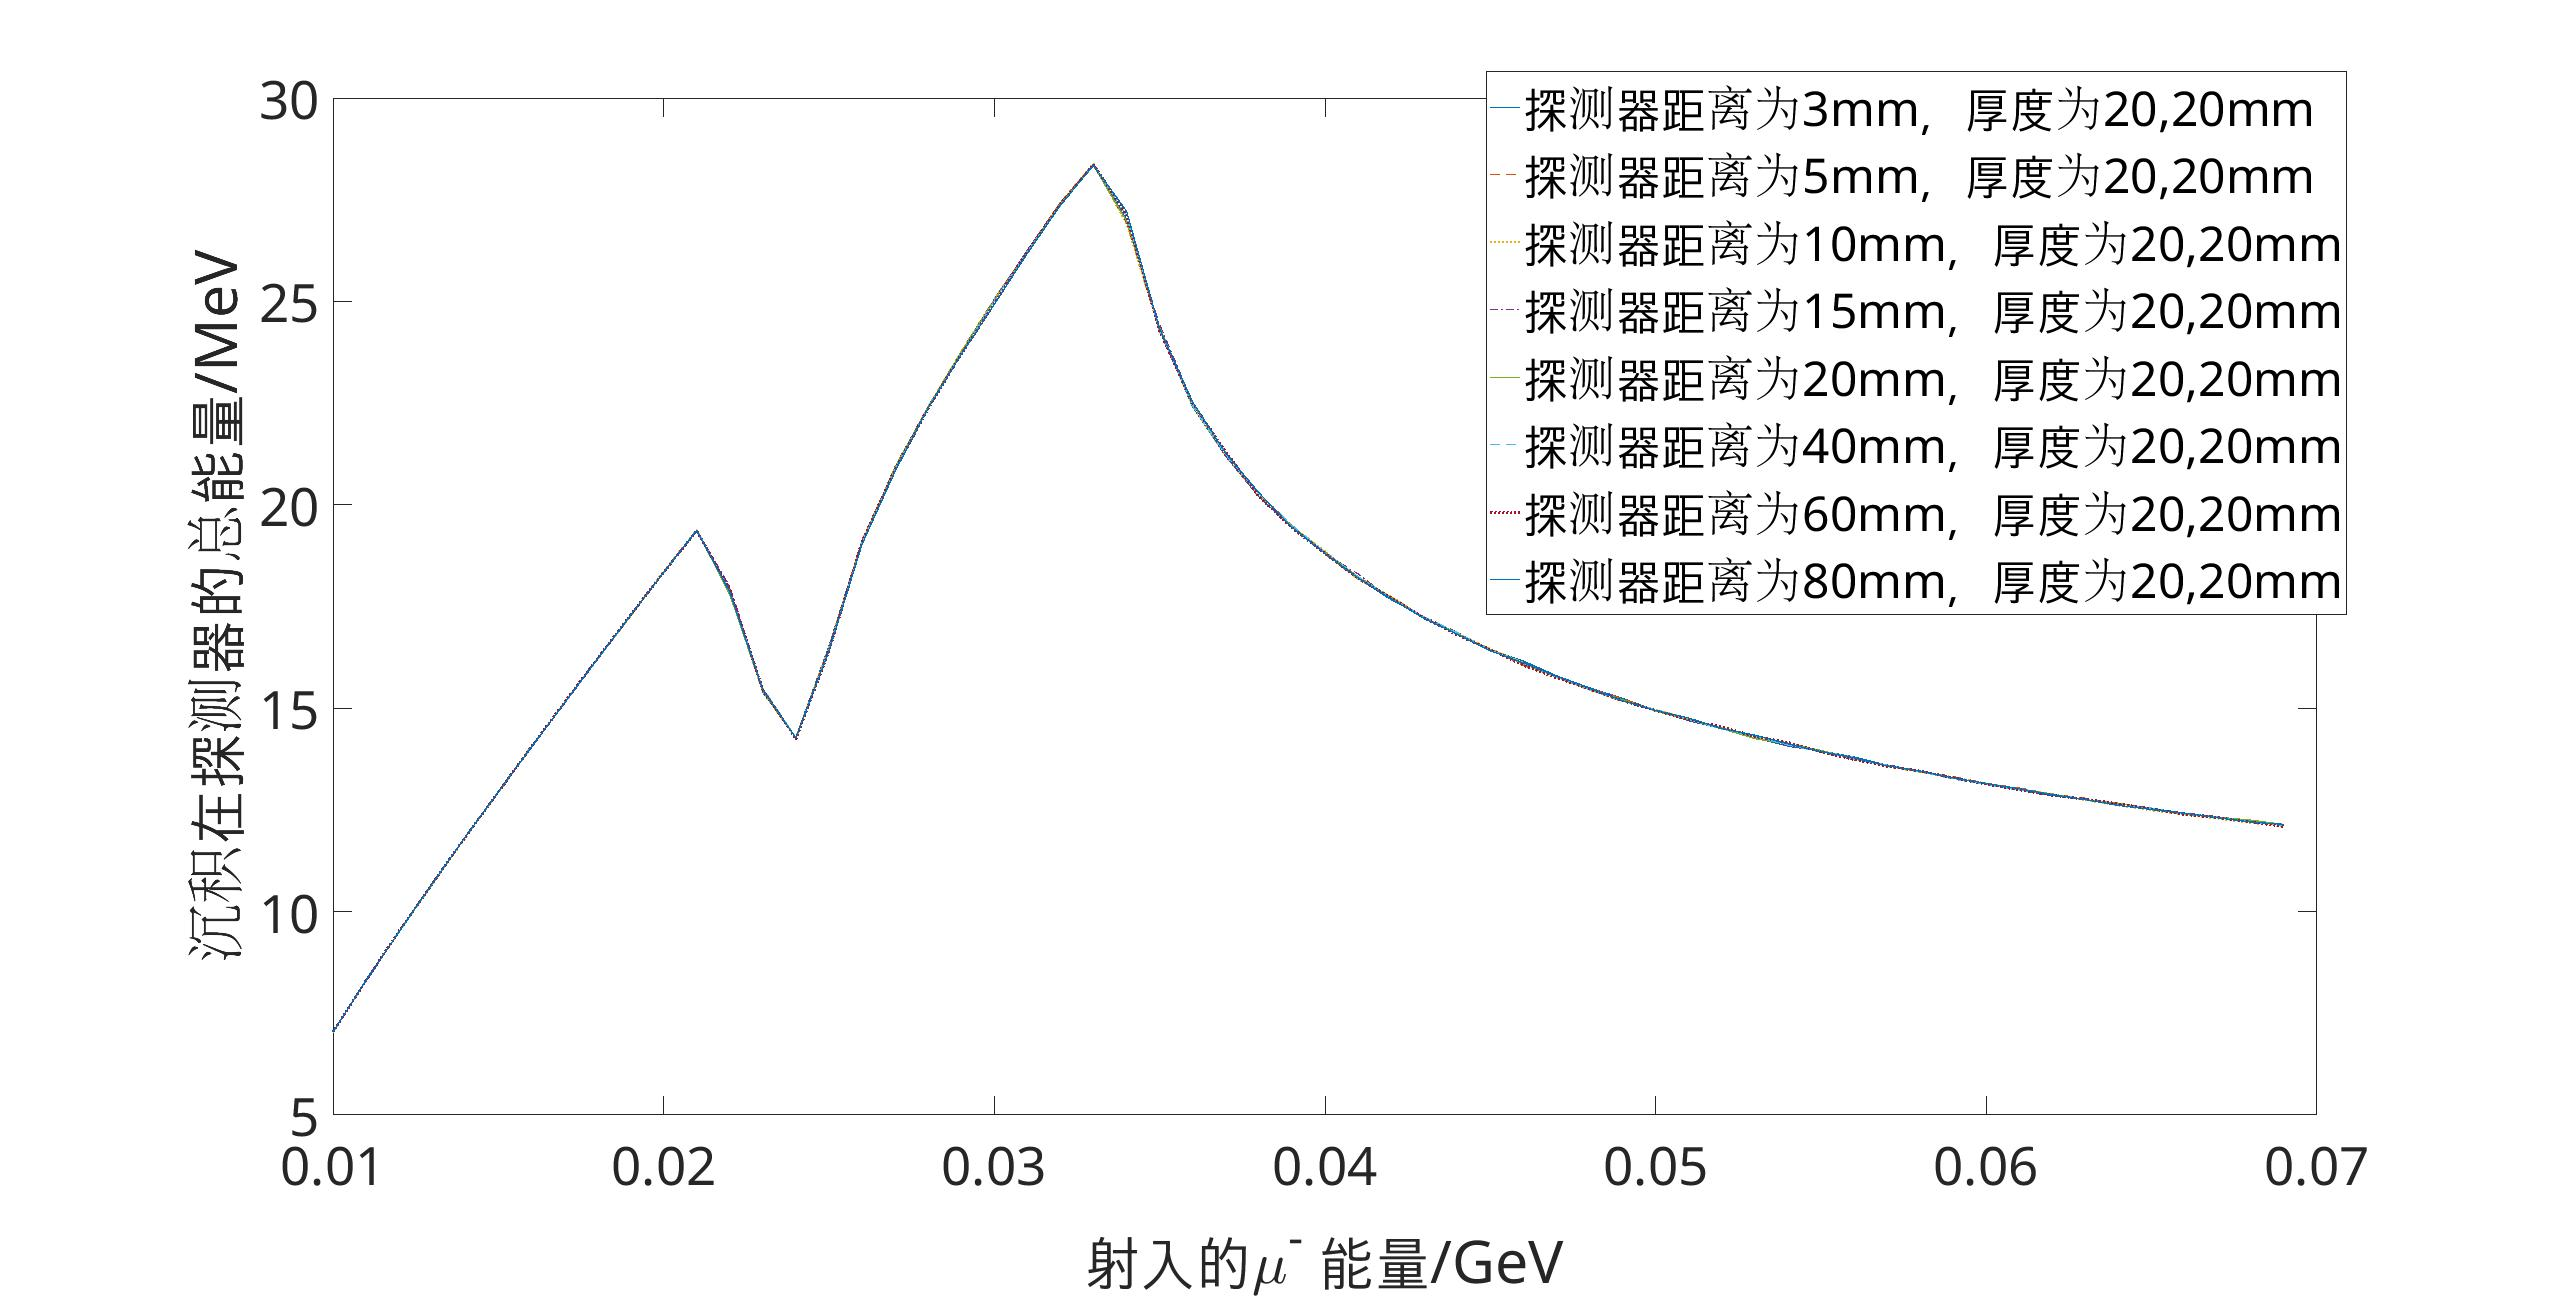
\includegraphics[width=120mm,height=60mm]{pic/en_all.jpg}
    \caption{距离不同的缪子沉积能量曲线}
    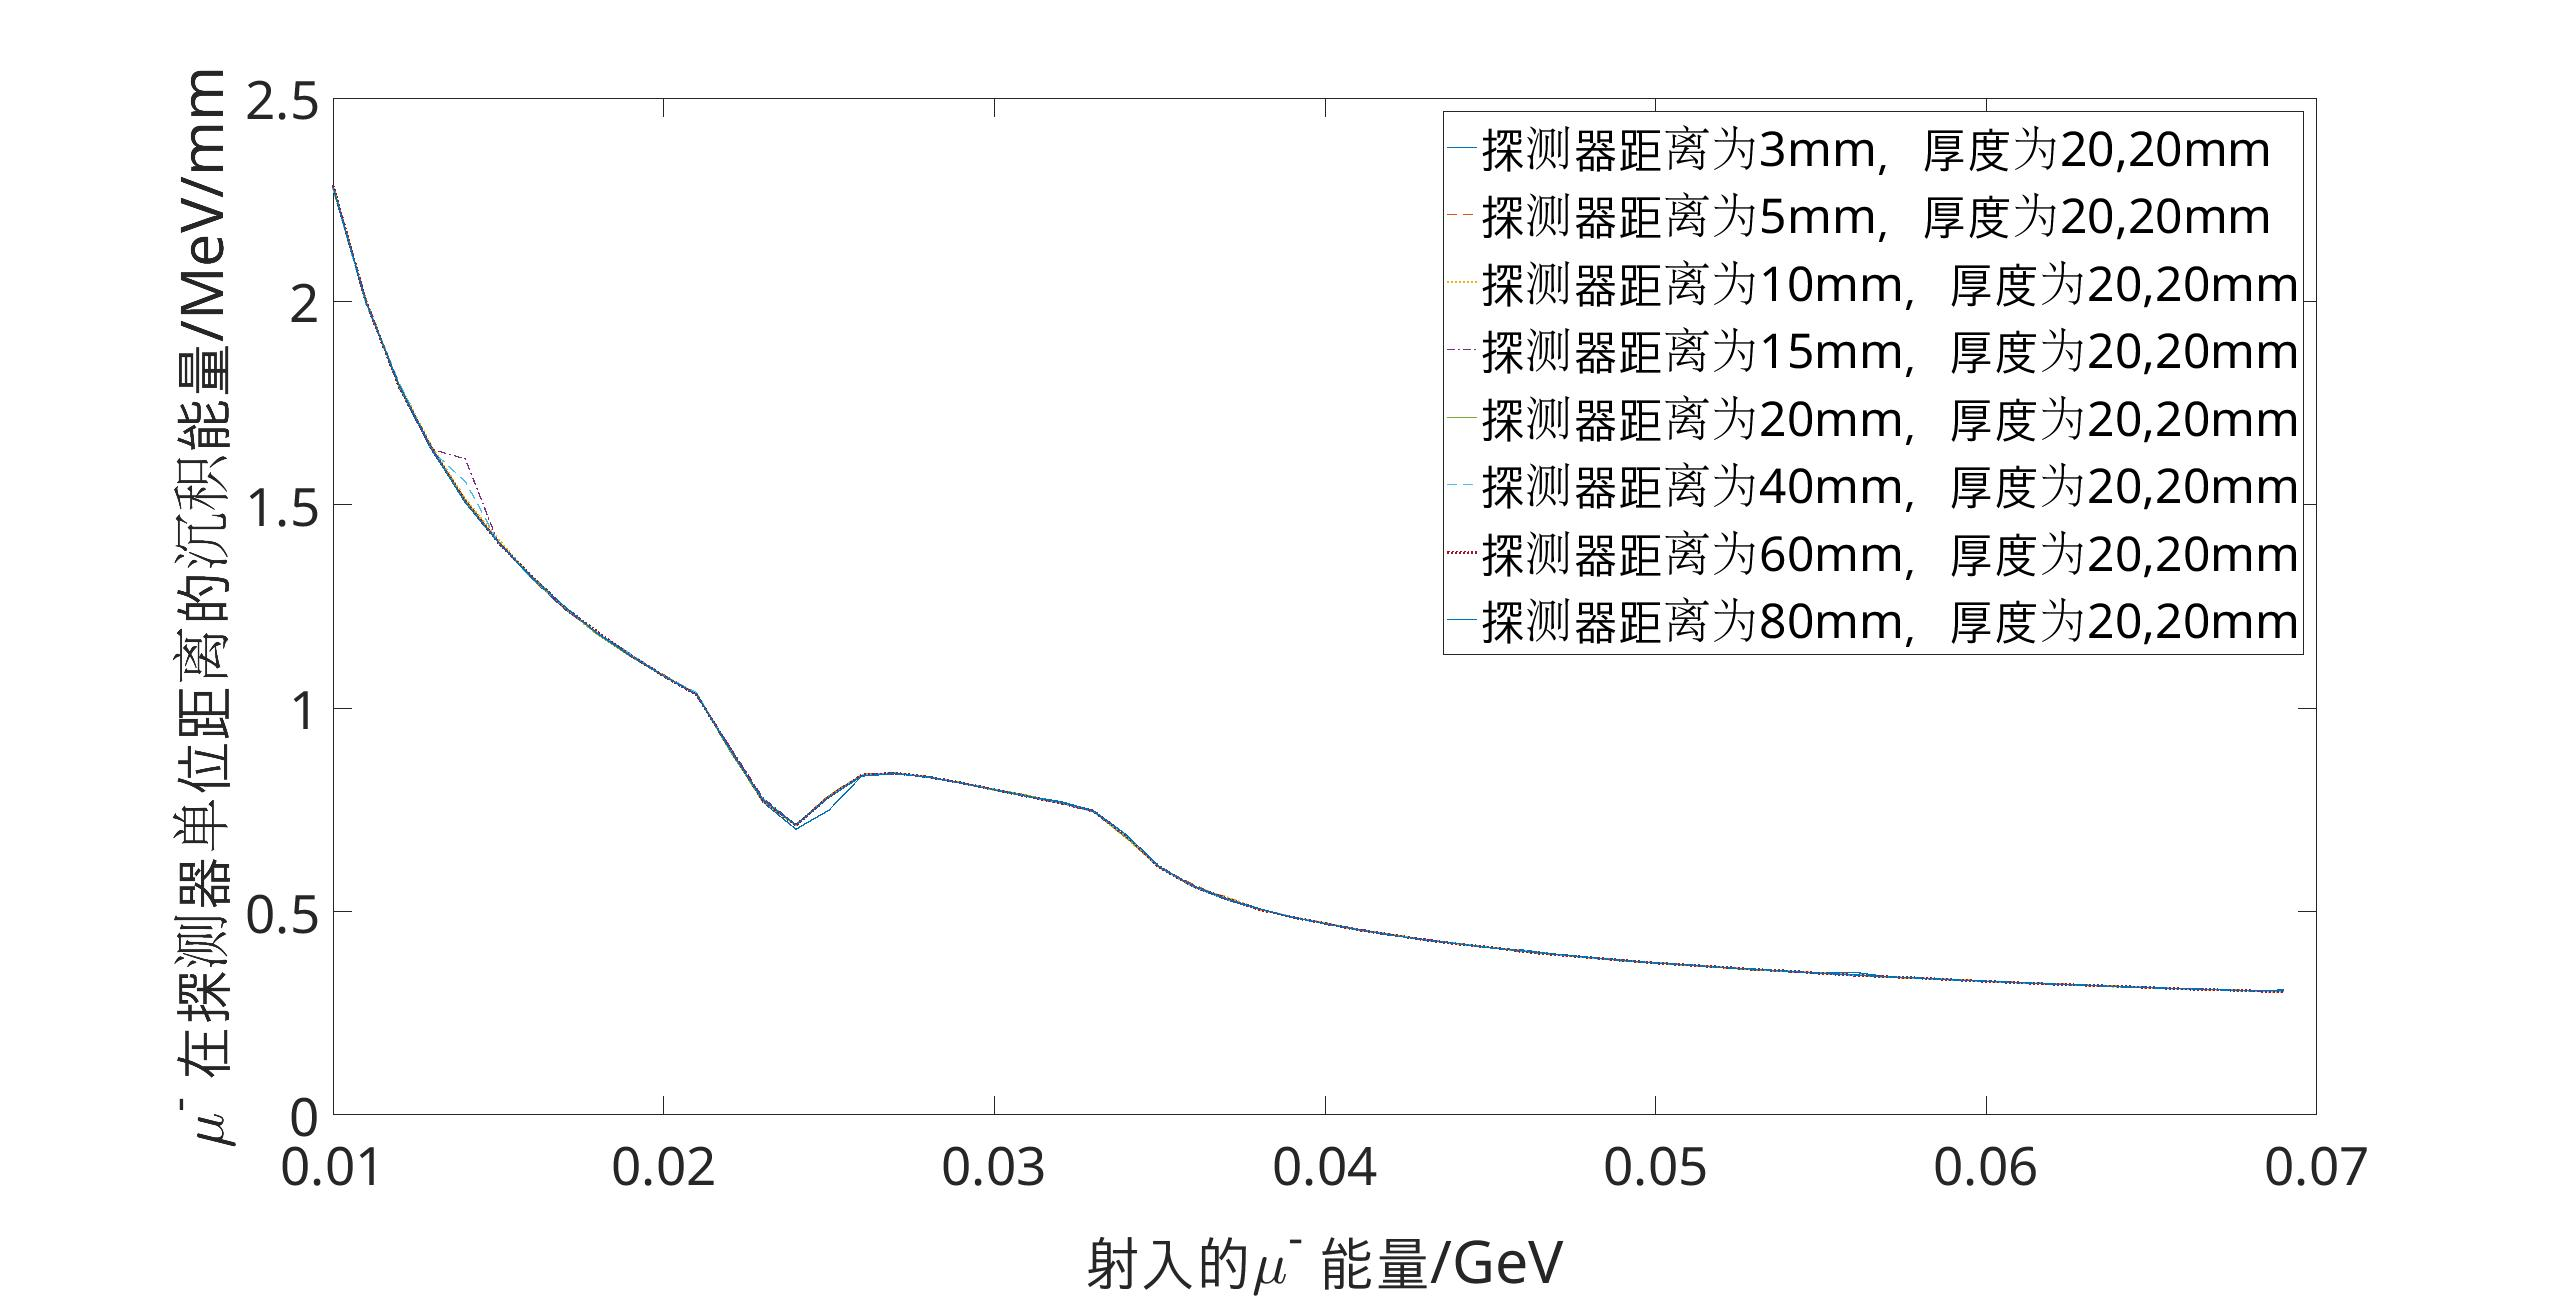
\includegraphics[width=120mm,height=60mm]{pic/en_dis_all.jpg}
    \caption{距离不同的缪子单位距离沉积能量曲线}
\end{figure}

\subsection{缪子衰变统计}

我们统计了每个事例中的缪子衰变产生的光子射出探测器的平均值,由于缪子达到探测器的时间只有几纳秒,所以我们直接用该时间表示差值,按间隔100ns 统计衰变时间得到如下拟合曲线\\

\begin{figure}[H]
\centering
    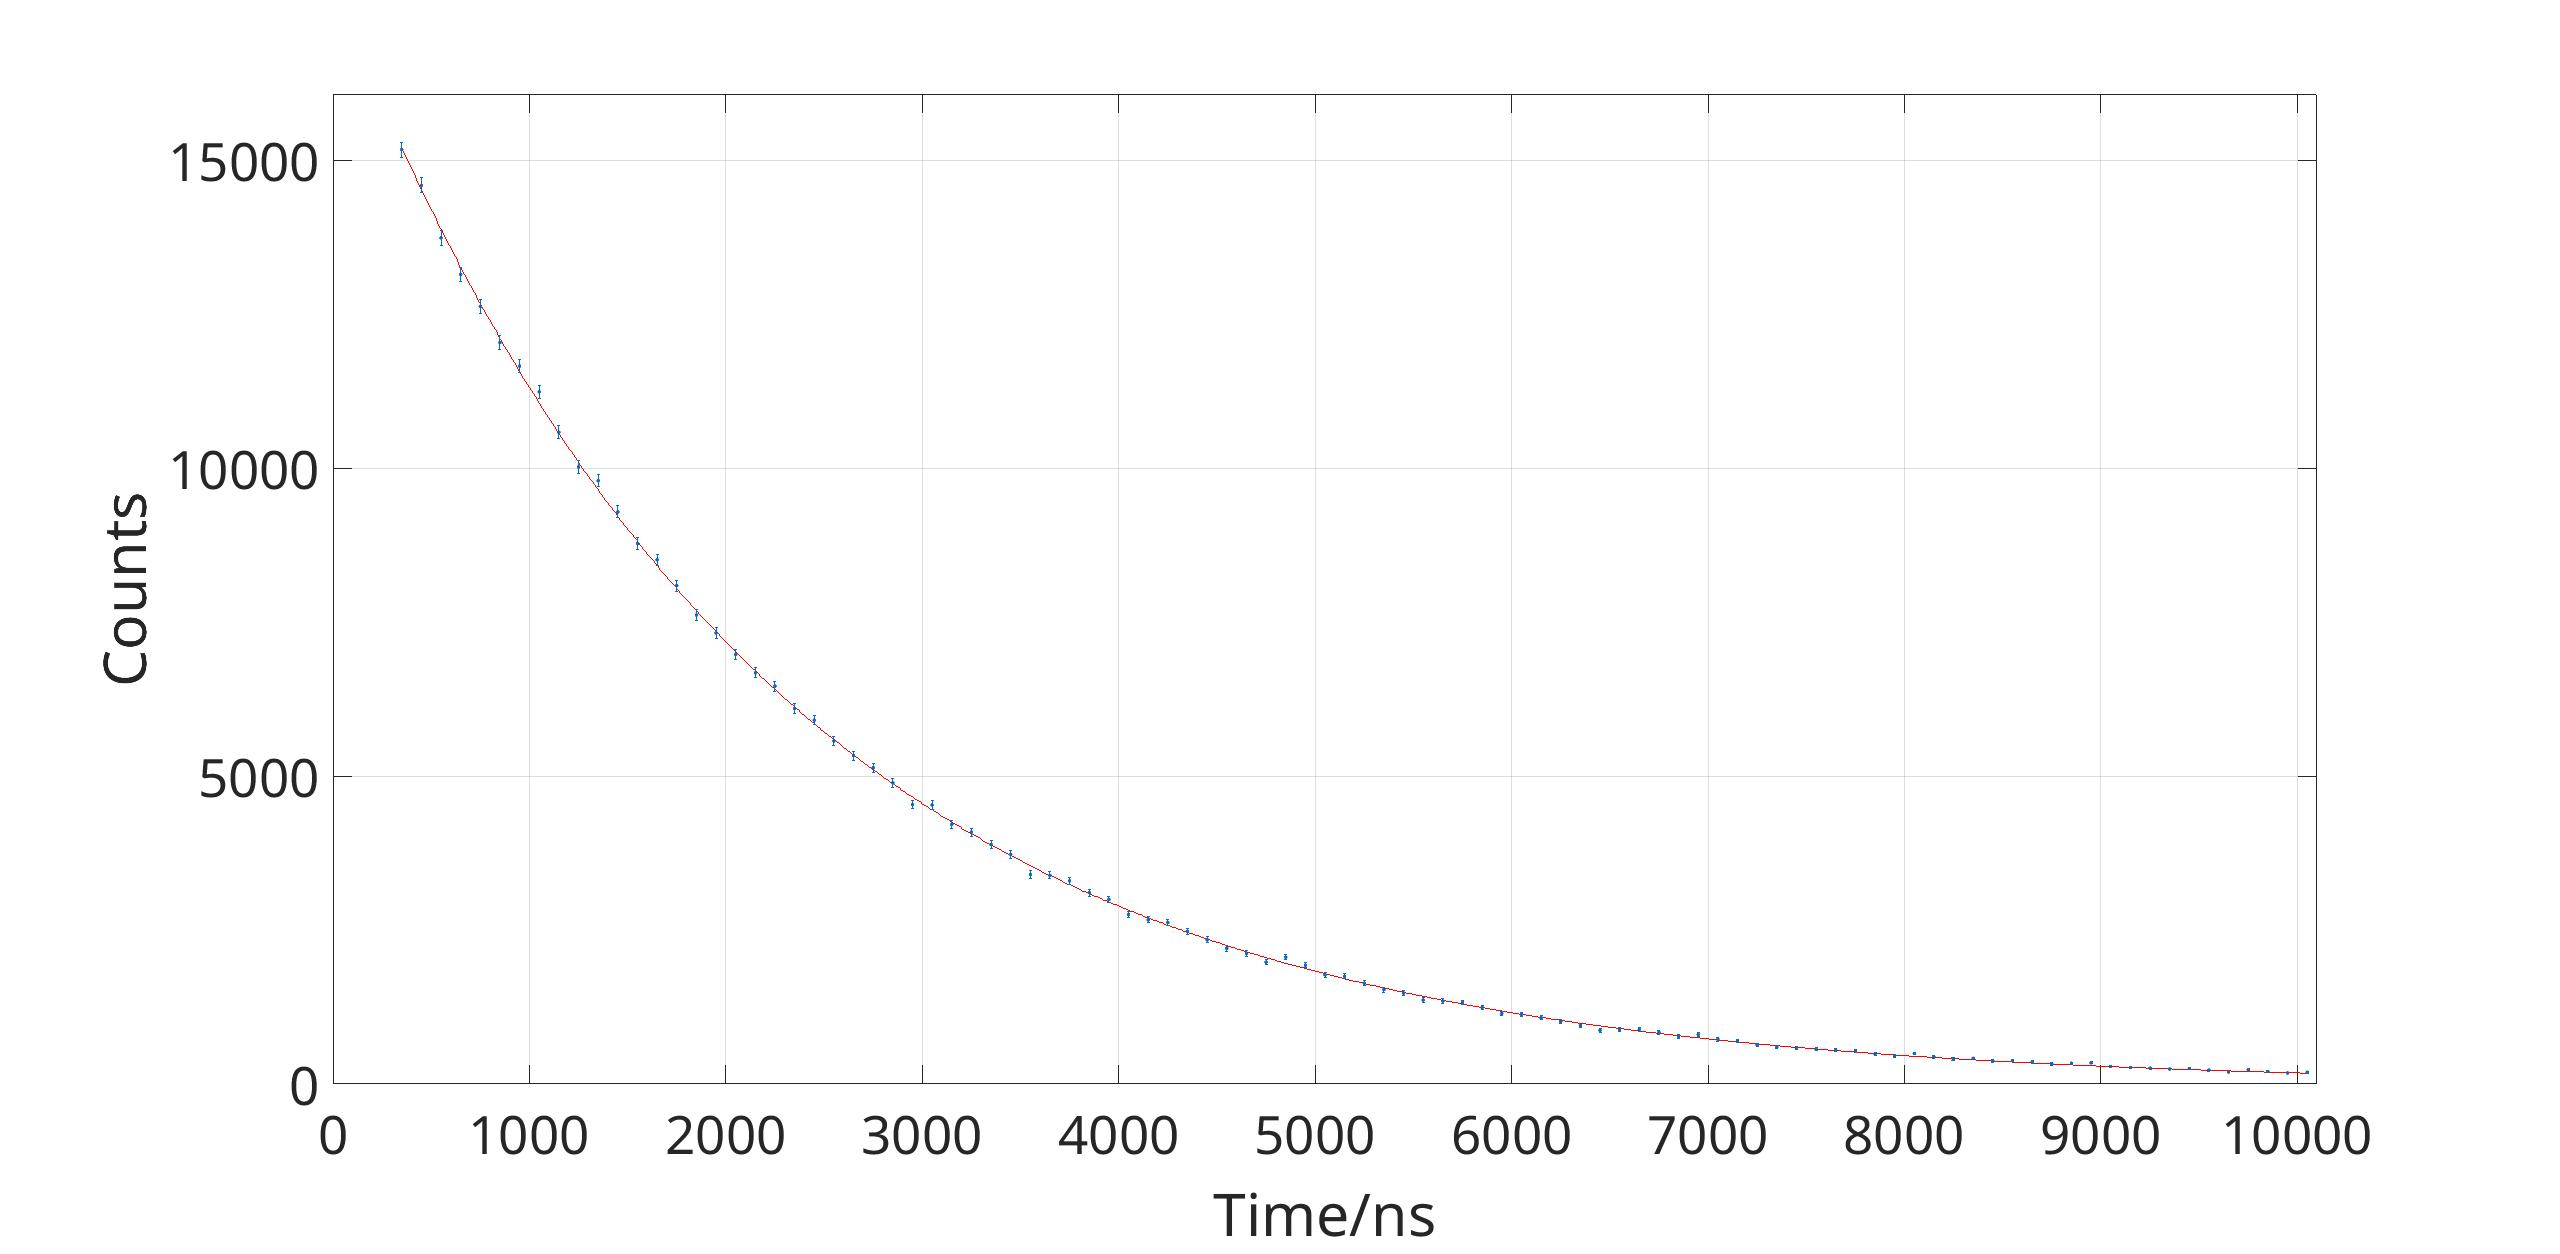
\includegraphics[width=120mm,height=60mm]{pic/counts.jpg}
    \caption{缪子衰变时间统计图}
\end{figure}

拟合曲线$ a\times exp(-1/b\times x)+c$的参数为\\
Coefficients (with\ 95\%\ confidence\ bounds):
\begin{align}
      a & = & 1.783e+04 & (1.777e+04, 1.789e+04)\\
       b & =  &    2203 & (2189, 2218)\\
       c & =  & -10.75 & (-33.95, 12.45)
\end{align}

sse: 2.5957e+05 rsquare: 0.9998  rmse: 52.2712\\
其中b就是缪子的寿命,得到精确值为2203.435477,与标准值相差0.2937\%



\newpage
\begin{thebibliography}{123456}
\bibitem {1}谢红刚, 牛胜利, 黄流兴. Geant4模拟半导体器件的单粒子效应[J]. 清华大学学报(自然科学版), 2007, 47(s1):1035-1039.
\bibitem {2}林延畅, 陈少敏, 高原宁,等. μ子寿命测量与高能物理实验创造性人才的培养[J]. 实验技术与管理, 2008, 25(9):34-37.
\bibitem {3}https://en.wikipedia.org/wiki/Muon
\bibitem {4}J. Beringer et al. (Particle Data Group), PR D86, 010001 (2012) (URL: http://pdg.lbl.gov)
\bibitem {5}吴雨生, 吕治严, 李数,等. 一种简便的$\mu$子寿命测量实验设计[J]. 中国科学技术大学学报, 2010, 40(6):608-611.
\end{thebibliography}
\end{document}